\documentclass[11pt,a4paper]{article}
\usepackage[margin=2.4cm]{geometry}
\usepackage{amsmath,amssymb,bm}
\usepackage{graphicx}
\usepackage{booktabs}
\usepackage{xcolor}
\usepackage[colorlinks=true,linkcolor=blue!50!black,citecolor=blue!50!black,urlcolor=blue!50!black]{hyperref}
\usepackage{caption}
\usepackage{natbib}
\captionsetup{font=small,labelfont=bf}

\newcommand{\pend}[1]{\textcolor{red}{[#1]}}
\newcommand{\exref}[1]{\textsf{\small #1}}
\newcommand{\dd}{\mathrm{d}}
\newcommand{\T}{^{\mathsf{T}}}
\newcommand{\Ni}{\mathsf{N}^{-1}}
\newcommand{\M}{\mathsf{M}}
\newcommand{\A}{\mathsf{A}}
\newcommand{\Pm}{\mathsf{P}}
\newcommand{\J}{\mathsf{J}}
\newcommand{\Tm}{\mathsf{T}}
\newcommand{\bs}{\beta_{\mathrm{s}}}
\newcommand{\nuref}{\nu_{\mathrm{ref}}}
\newcommand{\nupiv}{\nu_{\mathrm{piv}}}
\newcommand{\chimin}{\chi^2_{\min}}
\newcommand{\muK}{\mu\mathrm{K}}
\newcommand{\E}{\mathrm{E}}
\newcommand{\Var}{\mathrm{Var}}
\newcommand{\tr}{\mathrm{tr}}

\title{\Large Spectral indices and incidental amplitudes in pixel-based Bayesian component separation:
tempered samplers, reference-frequency priors, and the polarized synchrotron index of the public
WMAP and Planck maps}
\author{T.~L.~Svalheim\\[2pt]
{\small Draft of \today. Internal, not for distribution. Every number carries the identifier of the
experiment record it comes from, in the form \exref{E035}; records are in \texttt{nextgen/experiments/}.}}
\date{}

\begin{document}
\maketitle

\begin{abstract}
\noindent
In pixel-based Bayesian component separation a few spectral indices share the data with a very large
number of per-pixel amplitudes. We study what three common ways of removing the amplitudes do to
the index. (1) A Metropolis move that proposes an index, redraws the amplitudes and accepts on the
$\chi^2$ of the new pair is, on its own, a pseudo-marginal kernel for the profile posterior; inside a
Gibbs sweep that also redraws the amplitudes it becomes Monte Carlo within Metropolis and, for small
steps, converges to the profile posterior raised to the power $1/T$, with $T = \tfrac12 + 1/(4c_k)
\simeq \sqrt{\pi k/8} + \tfrac12$ for $k$ amplitudes. The index error from such a chain is too wide by
$0.79\,k^{1/4}$. We derive the law and its form for several moves per amplitude draw and for inexact
stored amplitudes, and confirm it against an exact-kernel calculation and simulated chains within
their Monte Carlo errors of 0.4 percent. (2) Moving the frequency at which a flat amplitude prior is
stated multiplies the index prior by an exponential with rate $n\ln(\nu_{\rm ref}'/\nu_{\rm ref})$,
$n$ the number of amplitudes. For one component the index is shifted by
$\ln(\nu_{\rm ref}/\nu_{\rm piv})$ times the index variance carried by one amplitude, a shift that
does not average down over pixels, changes sign across a pivot frequency set by the bands and by the
prior on the CMB, and has opposite signs for references of 23 and 30 GHz with the WMAP and Planck
LFI bands. (3) The profile likelihood has an exactly unbiased score, but its curvature is too sharp
by $\sqrt{1+\Tm/\J}$, where $\Tm/\J$ is the inverse mean squared signal-to-noise ratio of the amplitudes;
the natural plug-in sandwich correction is biased the wrong way, and a debiased form gives nominal
coverage over four decades of $\Tm/\J$. For one component and a uniform noise pattern a zero-mean
amplitude prior with a free scale is the same estimator; otherwise it is biased by up to 0.6 standard
deviations. We then apply the estimators side by side to the WMAP nine-year K to V polarization maps
with their dense noise covariances. On the same maps, regions and noise model the high-latitude
polarized synchrotron index is $-3.09$ with the profile likelihood, $-3.10$ with a flat amplitude
prior stated at 23 GHz and $-2.94$ with the same prior stated at 30 GHz, twelve statistical standard
deviations from a change of convention, as the identity predicts to 8 percent; for a band set
without K band and with a free CMB amplitude the same change of convention moves it by more than a
unit. We do not quote an index: at the statistical precision of these maps (0.01 to 0.02) it also
moves by 0.02 to 0.09 with the angular scales that inform it and with the band subset, and the
official Planck 30 GHz polarization maps do not fit one power law with WMAP K band.
\end{abstract}

\section{Introduction}

Bayesian component separation in the pixel domain fits, in every pixel, the amplitude of each sky
component, and for the whole sky or for large regions a small number of spectral parameters that say
how each component scales with frequency. In the Gibbs samplers that the Planck, BeyondPlanck and
Cosmoglobe analyses are built on \citep{eriksen2008,svalheim2023,watts2023}, the two kinds of
parameter are updated in turn. The amplitudes are many and each is poorly determined; the spectral
indices are few and are what the cleaning of large-scale polarization, and therefore the optical
depth to reionization, depends on. The published polarized synchrotron indices from the same public
maps span $-2.9$ to $-3.3$ depending on region, band set and method
\citep{dunkley2009,fuskeland2014,svalheim2023,weiland2022}, which is larger than their quoted errors.

This paper is about the statistical step that sits between the maps and such an index: how the
amplitudes are removed. That step has three places where it can go wrong without any error message,
and we treat them in turn.

\emph{The sampler} (Sect.~\ref{sec:legacy}). A move that proposes a new index, re-solves the
amplitudes and accepts on the $\chi^2$ of the new pair looks like a way to move both together. We
show that on its own it is a valid pseudo-marginal kernel for the profile posterior, that the
amplitude step of the Gibbs sweep turns it into Monte Carlo within Metropolis, and that the chain
then converges to the profile posterior raised to the power $1/T$ with
$T = \sqrt{\pi k/8} + \tfrac12$ for $k$ amplitudes. The index error bar from such a chain is too wide
by $0.79\,k^{1/4}$, a factor 16 for the $1.9\times10^5$ amplitudes of an $N_{\rm side}=64$ analysis,
with an acceptance rate that stays near one half.

\emph{The prior} (Sect.~\ref{sec:flat}). With flat priors on the amplitudes, the standard choice, the
index posterior contains the volume of amplitude space. This is known to bias indices
\citep{eriksen2008,dunkley2009,alonso2017}. We show that it is exactly equivalent to an exponential
prior on the index whose rate is the number of amplitudes times the logarithm of the reference
frequency at which the amplitudes are defined, give the resulting shift in closed form, and show that
its sign flips between the two reference frequencies in common use, 23 and 30 GHz, for the WMAP and
LFI bands when the CMB amplitude is constrained (with a free CMB amplitude both pull the index flat).
The shift does not shrink as pixels are added.

\emph{The error bar} (Sect.~\ref{sec:profile}). The profile likelihood has neither problem and its
score is exactly unbiased, but its curvature understates the error where the amplitudes are faint.
We give the correction in closed form, show that the obvious way to evaluate it on real data is
biased in the wrong direction, give the version that is not, and show its coverage over four decades
of the controlling ratio. A zero-mean amplitude prior with a free scale turns out to be the same
estimator when the noise pattern is uniform, and a biased one when it is not.

Sect.~\ref{sec:data} applies the estimators side by side to the WMAP nine-year $K$ to $V$ band
polarization maps with their released dense noise covariances, on regions defined by geometry with
the brightest emission masked, so that the difference between their answers is the difference between
the estimators. It then lists what else moves the index on these maps and by how much, where the
model with one power law per region passes and where it fails, and why we give the indices as the
answer of that model and not as a measurement. Sect.~\ref{sec:limits} states where the
recommended estimator stops being enough, and Sect.~\ref{sec:impl} describes the implementation and
its tests. All results are for maps-only analyses at low resolution with amplitudes that enter
linearly; we do not treat the time-ordered data.

\section{Model, notation and the index targets in use}
\label{sec:model}

\subsection{Data model}

The data are maps $d_b$ in bands $b = 1,\dots,n_{\rm b}$, each a vector over elements $p$ (pixels,
and Stokes parameters in polarization), in thermodynamic units. The parametric model is
\begin{equation}
  d_b = \sum_c m_{b,c}(\beta)\, a_c + n_b , \qquad n_b \sim \mathcal{N}(0, \mathsf{N}_b),
  \label{eq:model}
\end{equation}
with one amplitude $a_c(p)$ per component $c$ and element, a mixing coefficient $m_{b,c}$ that is the
component spectrum averaged over the bandpass of band $b$, and spectral parameters $\beta$ that are
shared by many elements: one value for the sky, one per region, or a field at lower resolution than
the amplitudes. Stacking bands and components, $d = \M(\beta)\,a + n$ with $a$ of length $k$. We write
\begin{equation}
  \A = \M\T \Ni \M , \qquad \hat a = \A^{-1} \M\T \Ni d , \qquad
  \Pm = \Ni - \Ni \M \A^{-1} \M\T \Ni ,
\end{equation}
all functions of $\beta$, so that
\begin{equation}
  \chi^2(\beta, a) = \chimin(\beta) + (a - \hat a)\T \A\, (a - \hat a), \qquad \chimin(\beta) = d\T \Pm d .
  \label{eq:chisplit}
\end{equation}
For the power-law component that carries the index, $m_{b}(\beta)$ is the band average of
$(\nu/\nuref)^{\beta}$ in brightness temperature, converted to thermodynamic units, so that the
amplitude is the brightness temperature at the reference frequency $\nuref$. The reference frequency
is a convention: it changes the meaning of $a$ and not the model.

The amplitudes are what statisticians call incidental parameters \citep{neyman1948}: their number
grows with the data, and the parameters of interest, the indices, are few. Everything in this paper
is a consequence of how the incidental parameters are removed.

\subsection{Four ways to remove the amplitudes}

\paragraph{Joint posterior with flat amplitude priors.} With $p(a) \propto 1$ the joint posterior is
$p(\beta)\exp[-\chi^2(\beta,a)/2]$ and integrating Eq.~(\ref{eq:chisplit}) over $a$ gives the index
marginal
\begin{equation}
  \mathcal{L}_{\rm flat}(\beta) \propto \exp\!\left[-\tfrac12 \chimin(\beta)\right] \det \A(\beta)^{-1/2} .
  \label{eq:Lflat}
\end{equation}
A Gibbs sampler that draws $a \mid \beta$ with its fluctuation and then moves $\beta$ on $\chi^2$ at
fixed $a$ has exactly this marginal for $\beta$, whether or not it mixes well enough to show it
(checked numerically and re-derived independently, \exref{E012}). The determinant is the volume
of amplitude space allowed at a given $\beta$. It is an implicit prior on the index and the subject of
Sect.~\ref{sec:flat}.

\paragraph{Profile likelihood.} Maximizing over the amplitudes instead of integrating gives
\begin{equation}
  \mathcal{L}_{\rm prof}(\beta) \propto \exp\!\left[-\tfrac12 \chimin(\beta)\right],
  \label{eq:Lprof}
\end{equation}
the spectral likelihood of \citet{stompor2009} (their Eq.~9; their Eq.~10 is the marginal form).
As a Bayesian target it is the marginal under the amplitude prior
$p(a \mid \beta) \propto \det \A(\beta)^{1/2}$, a Jeffreys prior for the amplitude block conditional on
the index. It is not the marginal under the joint Jeffreys prior of $(a, \beta)$, which depends on $a$.

\paragraph{Gaussian amplitude prior.} With $a \sim \mathcal{N}(\mu, \mathsf{S})$ the marginal keeps the
form of Eq.~(\ref{eq:Lflat}) with $\A \to \A + \mathsf{S}^{-1}$ and the prior mean entering $\chimin$.
We use two cases. A zero-mean prior with one free scale per index region,
$a_{\rm s}(p) \sim \mathcal{N}(0, \tau_r^2)$ for $p$ in region $r$, with $\tau_r$ maximized or
marginalized under a prior flat in $\ln\tau_r$. And, for intensity, a prior whose mean and scale are
tied to a template, with hyperparameters inferred. Under a change of reference frequency $\tau_r$
rescales by $(\nuref'/\nuref)^{\beta_r}$, and both maximization and a log-flat prior are invariant
under that rescaling, so the first case does not depend on the reference frequency.

\paragraph{Re-solving the amplitudes inside the index move.} A fourth route is procedural: propose
$\beta'$, solve for new amplitudes at $\beta'$, and accept on the $\chi^2$ of the new pair. What this
samples depends on how the new amplitudes are produced, and is the subject of
Sect.~\ref{sec:legacy}.

\subsection{Information and score}

Let $\M_r = \partial \M/\partial\beta_r$ for index parameter $r$. For data that follow
Eq.~(\ref{eq:model}) with true amplitudes $a$, the profile score
$s_r = -\tfrac12\,\partial\chimin/\partial\beta_r$ has zero mean and covariance
\begin{equation}
  \mathrm{Cov}(s_r, s_{r'}) = \J_{rr'} + \Tm_{rr'}, \qquad
  \J_{rr'} = (\M_r a)\T \Pm\, (\M_{r'} a), \qquad
  \Tm_{rr'} = \tr\!\left(\A^{-1} \M_r\T \Pm\, \M_{r'}\right),
  \label{eq:JT}
\end{equation}
while the expected curvature of $\tfrac12\chimin$ is $\J$ alone (derivation in
App.~\ref{app:sandwich}). $\J$ is the Fisher information on the indices with the amplitudes
profiled out. $\Tm$ does not depend on the signal: it is the part of the score variance that the
noise in the fitted amplitudes contributes. For one power-law component, diagonal noise with weights
$w_{pb} = 1/\sigma_{pb}^2$ and one region, these reduce to
\begin{equation}
  \J = \sum_p u_p V_p, \qquad \Tm = \sum_p V_p, \qquad
  u_p = a_p^2 \sum_b w_{pb} m_b^2, \qquad
  V_p = \mathrm{Var}_{w m^2}(\ln \nu)_p ,
  \label{eq:uV}
\end{equation}
with $u_p$ the squared signal-to-noise ratio of amplitude $p$ and $V_p$ the variance of $\ln\nu$ over
the bands under the weights $w_{pb} m_b^2$: the lever arm.

\section{What the re-solve move converges to}
\label{sec:legacy}

\subsection{The move}

The move we analyse is natural, and a version of it was the spectral-index step of the per-pixel
path in the development version of Commander4 that we started from (option
\texttt{resolve\_chisq} in our branch). Given the current $(\beta, a)$:
\begin{enumerate}
  \item propose $\beta'$ from a symmetric random walk;
  \item draw new amplitudes from their conditional at the proposed index,
        $a' \sim \mathcal{N}\!\big(\hat a(\beta'), \A(\beta')^{-1}\big)$;
  \item accept $(\beta', a')$ with probability $\min\{1, \exp[-(\chi^2(\beta',a') - \chi^2(\beta,a))/2]\}$.
\end{enumerate}
The Gibbs sweep then continues with the amplitude group, which redraws
$a \sim \mathcal{N}(\hat a(\beta), \A(\beta)^{-1})$, and possibly repeats the index move $n$ times before
that. The intent is to move the index and the amplitudes together and so avoid the slow mixing of the
conditional index step. Write $X = (a-\hat a)\T \A (a-\hat a)$, so that
$\chi^2 = \chimin(\beta) + X$ by Eq.~(\ref{eq:chisplit}). For an amplitude draw from the conditional,
$X \sim \chi^2_k$ whatever $\beta$ is.

\subsection{Alone, the move is exact for the profile posterior}

Because $\E[\exp(-X/2)] = 2^{-k/2}$ does not depend on $\beta$, the quantity
$\exp[-\chi^2(\beta, a)/2]$ at a fresh conditional draw is an unbiased estimator of
$\mathcal{L}_{\rm prof}(\beta)$ up to a constant. Steps 1 to 3, with the accepted amplitudes kept as
part of the state, are therefore a pseudo-marginal Metropolis-Hastings kernel
\citep{beaumont2003,andrieu2009}. Its extended target is
\begin{equation}
  \pi(\beta, a) \propto p(\beta)\, \exp\!\left[-\tfrac12\chimin(\beta)\right]\,
  \det\A(\beta)^{1/2} \exp\!\left[-(a-\hat a)\T \A\, (a-\hat a)\right],
  \label{eq:extended}
\end{equation}
whose index marginal is the profile posterior and whose amplitude conditional is
$\mathcal{N}(\hat a, (2\A)^{-1})$: the amplitudes carry half their posterior covariance. So the move
does have a target, the target is the profile posterior, and the determinant never enters. This is why
chains run with this move have means close to the profile posterior. Under
Eq.~(\ref{eq:extended}), $X \sim \mathrm{Gamma}(k/2, 1)$ with mean $k/2$.

\subsection{The amplitude step of the Gibbs sweep breaks it}

The amplitude group redraws $a$ with the full conditional covariance $\A^{-1}$, which resets $X$ to a
$\chi^2_k$ variate with mean $k$. That is the conditional of the flat-prior joint posterior and not of
Eq.~(\ref{eq:extended}). The two kernels share no invariant distribution. With one index move per
amplitude draw, both the current and the proposed estimate are fresh at every index move, and the
composite is Monte Carlo within Metropolis in the terminology of \citet{andrieu2009}, following
\citet{oneill2000} and \citet{beaumont2003}. \citet{andrieu2009} note that the target is typically
not the invariant density of such a chain and that the existence of an invariant distribution is not
obvious in general. Here it can be written down.

\subsection{The stationary law: a tempered profile posterior}

With one move per amplitude draw the index chain is Markov on its own, with acceptance probability
\begin{equation}
  \alpha(D) = \E\big[\min\{1, e^{-(D+Z)/2}\}\big], \qquad
  D = \chimin(\beta') - \chimin(\beta) - 2\ln\frac{p(\beta')}{p(\beta)}, \qquad Z = X' - X ,
\end{equation}
where $X$ and $X'$ are independent $\chi^2_k$ variates, so $Z$ is symmetric with variance $4k$. In the
limit of small proposal steps the chain is a diffusion with drift proportional to $\alpha'(0)$ and
diffusion coefficient proportional to $\alpha(0)$, and its stationary density is
\begin{equation}
  \pi(\beta) \propto \left\{ p(\beta) \exp\!\left[-\tfrac12\chimin(\beta)\right] \right\}^{1/T},
  \qquad T = \frac12 + \frac{1}{4 c_k}, \qquad
  c_k = \E\big[e^{-Z/2};\, Z > 0\big] = 2^{-(k+1)} \binom{k}{k/2} .
  \label{eq:Tk}
\end{equation}
The formula is exact for every $k$ and every shape of $\chimin$ in the small-step limit; $T(0) = 1$
recovers Metropolis. For large $k$,
\begin{equation}
  T = \sqrt{\frac{\pi k}{8}} + \frac12 + O(k^{-1/2}) ,
  \label{eq:Tlarge}
\end{equation}
so the index posterior is the profile posterior with its width multiplied by
$\sqrt{T} \simeq 0.79\, k^{1/4}$. The stationary acceptance rate is $\tfrac12 + c_k$, close to one half
and independent of the step size, which is why such a chain looks healthy.

Equation~(\ref{eq:Tk}) does not need $\chi^2_k$ noise. For any symmetric acceptance noise $Z$ with
density $f_Z$, $T \simeq \tfrac12 + 1/(8 f_Z(0))$, and for Gaussian noise
\begin{equation}
  T \simeq \frac12 + \sqrt{\frac{\pi}{8}}\; \sigma_E , \qquad \sigma_E = \tfrac12\,\mathrm{sd}(Z) ,
  \label{eq:Tsigma}
\end{equation}
with $\sigma_E$ the standard deviation of the noise in the estimated energy difference, equal to
$1/\sqrt2$ times the standard deviation of the $\chi^2$ at a fresh amplitude draw. The leading term
is the effective temperature that \citet{ball2003} derived for the sign rule (accept if and only if
the noisy energy difference is negative; their Eq.~7), and that \citet{bardenet2017} recover without
assuming Gaussian noise (their Sect.~6.3). The Metropolis rule on the same noisy difference adds the
$\tfrac12$. Equation~(\ref{eq:Tsigma}) is the form to use when the stored amplitudes are not the drawn
ones, as below.

\paragraph{Several index moves per amplitude draw.} After the first accepted move the retained $X$ is
no longer fresh: it is biased low, and the next proposal has to beat it. In the large-$k$ limit the
accepted moves are the lower records of the sequence of fresh $X$ values, the $j$-th proposal after a
redraw is accepted with probability $1/(j+1)$, and the stationary law remains a power of the profile
posterior with temperature $T_n = R_n T_1$,
\begin{equation}
  R_n = \frac{H_{n+1} - 1}{\sqrt{\pi}\; N_\varphi(n)} , \qquad
  N_\varphi(n) = \sum_{j=1}^{n} j \int \varphi(t)^2\, [1 - \Phi(t)]^{\,j-1}\, \dd t ,
  \label{eq:Rn}
\end{equation}
where $H_n$ is the harmonic number, $\varphi$ and $\Phi$ are the standard normal density and distribution
function, and $N_\varphi(n)$ is the sum over proposals of the expected density at the running minimum.
$R_2 = 5/6$ exactly, and numerically
$R_n = 0.833$, $0.647$, $0.543$, $0.467$ and $0.357$ for $n = 2$, 5, 10, 20 and 100: more index
moves narrow the law only as $(\ln n)^{-1/4}$ in width, and the $k^{1/4}$ scaling is untouched.

\paragraph{The repair that is exact and useless.} Redrawing the amplitudes with half their covariance,
$a \sim \mathcal{N}(\hat a, (2\A)^{-1})$, is the conditional of Eq.~(\ref{eq:extended}) and makes the
composite exact for the profile posterior. Its acceptance rate at fixed index is
$2 I_{1/3}(k/2, k/2)$, with $I$ the regularized incomplete beta function, which decays as
$e^{-0.059 k}$: $6\times10^{-4}$ at $k = 100$. The useful repairs evaluate
Eq.~(\ref{eq:Lprof}) or Eq.~(\ref{eq:Lflat}) directly in the acceptance, which costs one extra
log-determinant per proposal at most (Sect.~\ref{sec:impl}).

\subsection{Tests}

\begin{table}
\centering
\caption{Variance of the stationary index distribution of the composite chain in units of the profile
posterior variance, one index move per amplitude draw, for $\chimin = \beta^2$ and exact $\chi^2_k$
refreshes. Columns: Eq.~(\ref{eq:Tk}); its leading term; the stationary vector of the exact kernel on
a grid of 1201 points, with the acceptance function computed by convolution of the $\chi^2_k$ density;
and a simulation of $10^4$ chains with a proposal step of $0.1\sqrt{T}$ (\exref{E035}, independent
review). The grid and the simulation sit 0.1 to 0.2 percent below the law because of the finite step.
Controls: with no refresh, or with a refresh from $\mathrm{Gamma}(k/2,1)$, the variance is $1.000 \pm
0.001$ at $k = 4$, 8 and 16.}
\label{tab:toy}
\begin{tabular}{rrrrrr}
\toprule
$k$ & $T$, Eq.~(\ref{eq:Tk}) & $\sqrt{\pi k/8}$ & exact kernel & simulation & acceptance \\
\midrule
10 & 2.532 & 1.982 & 2.524 & $2.525 \pm 0.008$ & 0.621 \\
100 & 6.782 & 6.267 & 6.769 & $6.751 \pm 0.024$ & 0.538 \\
1\,000 & 20.32 & 19.82 & 20.29 & $20.26 \pm 0.07$ & 0.511 \\
10\,000 & 63.17 & 62.67 & 63.07 & $63.30 \pm 0.23$ & 0.503 \\
100\,000 & 198.67 & 198.17 & 198.35 & $199.39 \pm 0.72$ & 0.500 \\
200\,000 & 280.75 & 280.25 & 280.31 & $280.22 \pm 1.01$ & 0.500 \\
\bottomrule
\end{tabular}
\end{table}

Table~\ref{tab:toy} and Fig.~\ref{fig:temper} compare Eq.~(\ref{eq:Tk}) with the exact kernel and with
simulated chains. The law was derived twice, the second time by an independent reviewer who was given
the algorithm and not our derivation. The two derivations agree, the reviewer's exact-kernel
calculation reproduces every row of our own toy within 1.4 standard errors, and the controls return
the profile posterior exactly, so the excess is caused by the full-covariance redraw and by nothing
else. For proposal steps that are not small the kernel is no longer reversible with respect to a
power of the profile posterior, but the variance stays within 8 percent of $T$ at any step size
(0.918 $T$ for steps of four stationary widths or more).

The same toy reproduces, within 5 percent, four earlier measurements of the width of chains run with
this move on simulated maps, with $k$ from 450 to 3072 and one or four moves per amplitude draw
(measured 3.9, 5.7, 3.2 and 4.4 profile widths; toy 4.0 to 4.1, 5.7, 3.0 and 4.3; \exref{E002},
\exref{E005}).

\paragraph{Real maps.} On nside-64 intensity maps (17 bands from Haslam to Planck 857 GHz, 38\,165
unmasked pixels, five components, so $k = 190\,825$; 20 index moves per amplitude draw) two chains
gave widths of 17.0 and 16.4 profile widths for the synchrotron index and 16.4 and 16.6 for the dust
index (\exref{E014}). The law with exact stored draws predicts 13.1 to 13.6 at these settings. The
difference has a specific cause. This code path stores the per-pixel amplitudes as spherical-harmonic
coefficients to $\ell_{\max} = 3 N_{\rm side} - 1$, and the $\chi^2$ in the acceptance is evaluated
on the round-tripped maps. The round trip is not exact on the HEALPix grid, so the stored amplitudes
differ from the drawn ones. The log of the run records the log acceptance ratio of every proposal,
and at the first move of each iteration both amplitude sets are fresh: the scatter of those 3200
values is $682 \pm 9$ where exact draws give $\sqrt{k} = 437$, a factor $2.44 \pm 0.06$ in variance. With
that one measured number in Eq.~(\ref{eq:Tsigma}) the toy gives widths of 15.9 and 16.6 and an
acceptance rate of 0.075, against the measured 0.074 and 0.077. The storage residual also has a
gradient in the dust index, which predicts a shift of the chain mean of $+3.1$ profile widths where
$+3.0 \pm 0.5$ was measured. A run of the same configuration with the amplitudes stored as maps is
predicted to give 13.1 and 13.6 widths and no shift; \pend{that run is not yet done}.

\begin{figure}
\centering
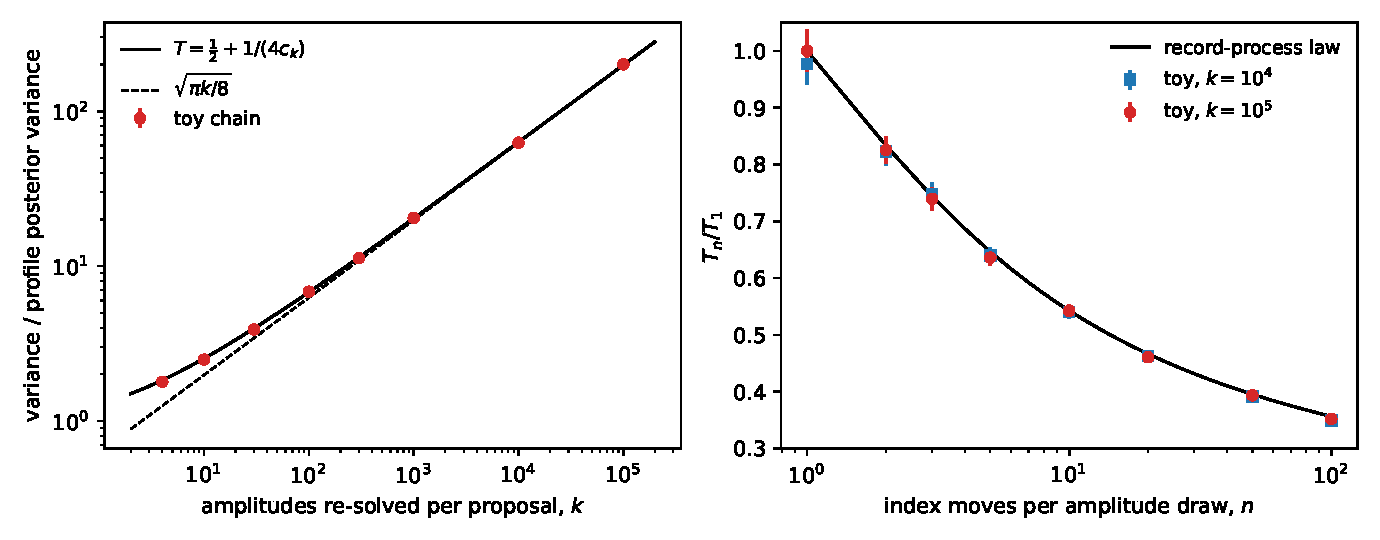
\includegraphics[width=0.98\textwidth]{figures/fig_temper.pdf}
\caption{The stationary law of the re-solve move inside a Gibbs sweep. Left: temperature of the
tempered profile posterior against the number of amplitudes re-solved per proposal, for one index
move per amplitude draw: Eq.~(\ref{eq:Tk}) (line), its leading term (dashed) and the toy chain
(points). Right: the ratio $T_n/T_1$ for $n$ index moves per amplitude draw: the record-process
law of Eq.~(\ref{eq:Rn}) (line) and the toy at $k = 10^4$ and $10^5$ (points).}
\label{fig:temper}
\end{figure}

\subsection{What this means for existing chains}

A chain run with this move reports index uncertainties that are too wide by $\sqrt{T}$, a factor of
order ten at map-level $k$, with a mean close to the profile posterior. It does not sample the
flat-prior joint posterior that the rest of the Gibbs sweep assumes. The statement applies to the
move as defined in steps 1 to 3 with exact conditional draws. Samplers that propose the index and
then solve for the conditional mean, or that evaluate a marginal likelihood in the acceptance, are
different algorithms. Commander3's index samplers are of the latter kinds (we read the code and did
not run it).

\section{The flat amplitude prior, written in terms of the reference frequency}
\label{sec:flat}

That the flat-prior marginal of Eq.~(\ref{eq:Lflat}) pulls spectral indices is known.
\citet{eriksen2008} found a global offset biased by more than $4\sigma$ under uniform priors and
removed it with a Jeffreys prior on the index. \citet{dunkley2009}, fitting one polarized synchrotron
index per $N_{\rm side}=2$ pixel to the five-year WMAP maps with uniform priors on the CMB and
synchrotron amplitudes defined at 23 GHz, found index posteriors centred on $-2.6$ in simulations,
noted that the effect grows with the number of pixels that share an index and that a Jeffreys prior
on the index does not remove it, and divided their prior by a factor estimated from a noise-only
simulation. \citet{alonso2017} cancel the determinant with a ``volume prior'', which in our reading
makes their target the profile likelihood, and show biases of more than $3\sigma$ without it. Jeffreys
or reference priors are used against prior-volume effects in several other analyses
\citep{dickinson2009,planck2015x,jew2019}, and \citet{andersen2023} describe the marginal and the
profile (``ridge'') index samplers of Commander, noting that the two differ by the determinant term. What has not been
written down, as far as we can find, is how large the pull is in closed form and what sets its sign.
Both follow from one identity.

\subsection{An exact identity}

Change the reference frequency of the power-law component from $\nuref$ to $\nuref'$. The mixing
column of every amplitude in index region $r$ is multiplied by $(\nuref/\nuref')^{\beta_r}$, so
$\M' = \M\,\mathsf{D}$ with $\mathsf{D}$ diagonal, $\chimin$ is unchanged, and
$\det\A' = \det\A \prod_r (\nuref/\nuref')^{2 n_r \beta_r}$, with $n_r$ the number of power-law
amplitudes in region $r$. Therefore
\begin{equation}
  \ln \mathcal{L}_{\rm flat}(\beta;\nuref') = \ln \mathcal{L}_{\rm flat}(\beta;\nuref)
  + \sum_r n_r\, \beta_r \ln\frac{\nuref'}{\nuref} ,
  \label{eq:tilt}
\end{equation}
for any number of components, any bandpasses and any noise covariance. Moving the frequency at which
a flat amplitude prior is stated is the same as multiplying the index prior by an exponential,
$e^{\lambda\beta}$ with $\lambda = n \ln(\nuref'/\nuref)$: 34 $e$-folds per unit of index for 128
amplitudes moved from 23 to 30 GHz. The profile likelihood and the zero-mean prior with a free scale
do not change.

\subsection{The shift and its pivot}

Let $g_r = -\tfrac12\,\partial \ln\det\A/\partial\beta_r$ be the gradient of the volume term. To first
order the maximum of $\mathcal{L}_{\rm flat}$ sits at the profile maximum plus
\begin{equation}
  \delta\beta = \mathsf{H}^{-1} g , \qquad
  \mathsf{H} = \J + \nabla\nabla\,\tfrac12\ln\det\A ,
  \label{eq:response}
\end{equation}
where $\mathsf{H}$ is the expected curvature of the flat-prior marginal itself: the profile information
plus the curvature of the volume term. For one power-law component with delta bands and diagonal
noise, $-\tfrac12 \ln A_p = \beta\ln\nuref - \tfrac12 \ln\sum_b w_{pb}\, \nu_b^{2\beta}$, so
\begin{equation}
  g = \sum_p \ln\frac{\nuref}{\bar\nu_p}, \qquad
  \ln\bar\nu_p = \frac{\sum_b w_{pb}\,\nu_b^{2\beta} \ln\nu_b}{\sum_b w_{pb}\,\nu_b^{2\beta}} , \qquad
  \nabla\nabla\,\tfrac12\ln\det\A = 2\sum_p V_p = 2\,\Tm ,
\end{equation}
where $\bar\nu_p$ is the frequency at which amplitude $p$ is best measured: the geometric mean of the
band frequencies under the weights (inverse noise variance times squared spectrum) that also define
the lever arm $V_p$ in Eq.~(\ref{eq:uV}). When the amplitudes of a region share a noise pattern,
$\bar\nu_p = \nupiv$ and, with $\sigma_\beta^2 = 1/\J$ the profile variance of the region index,
\begin{equation}
  \boxed{\;\delta\beta = \ln\!\left(\frac{\nuref}{\nupiv}\right) \frac{n\,\sigma_\beta^2}{1 + 2\,\Tm/\J}
         \;\longrightarrow\; \ln\!\left(\frac{\nuref}{\nupiv}\right) \sigma_1^2
         \quad (\Tm \ll \J)\;}
  \label{eq:shift}
\end{equation}
where $\sigma_1^2 = n\sigma_\beta^2$ is the index variance that a single amplitude carries, and
$\Tm/\J$ is the inverse mean squared signal-to-noise ratio of the amplitudes (Sect.~\ref{sec:profile}).
The boxed form is for one component. With further free amplitudes the curvature of the volume term
is no longer $2\Tm$ and can be negative, so that $\mathsf{H}$ is smaller than $\J$ and the flat-prior
marginal may have no interior optimum at all; one of our fits to real maps, for a band set without K band
and with a free CMB amplitude (on the earlier, unmasked regions described in Sect.~\ref{sec:data}), ends
at the edge of the allowed range (\exref{E040}). Three things follow.

\emph{The shift does not average down.} Adding amplitudes at fixed depth leaves $\sigma_1$ and
$\Tm/\J$ unchanged, so $\delta\beta$ stays the same while the posterior width falls as $n^{-1/2}$. In
units of the posterior width the pull grows as $\sqrt{n}$: this is the observation of
\citet{dunkley2009} that the effect increases with the number of pixels per index, and it is the
Neyman-Scott structure \citep{neyman1948}. More data of the same kind make it worse. So does a finer
pixelization of the same data: for $\Tm \ll \J$, four times as many amplitudes for the same region
information is four times the shift.

\emph{The sign is set by the convention.} The index is pulled steep if the reference lies below the
pivot and flat if above. A flat prior is neutral only when stated at the pivot.

\emph{The pivot depends on the other components and on their priors.} A component with a free
amplitude and a spectrum that does not depend on the index (the CMB, dust with fixed parameters)
contributes nothing to $g$ directly, but projecting it out replaces the weights $w_{pb}$ by the
projected weight matrix $\tilde{\mathsf{W}}_p = \mathsf{W}_p - \mathsf{W}_p \mathsf{F}
(\mathsf{F}\T\mathsf{W}_p\mathsf{F} + \mathsf{S}^{-1})^{-1}\mathsf{F}\T\mathsf{W}_p$, with $\mathsf{F}$ the spectra of the
other components and $\mathsf{S}$ their prior covariance. The pivot becomes a generalized mean under
$\tilde{\mathsf{W}}_p$, which has negative off-diagonal elements and can lie outside the range of the
bands. With a free CMB amplitude under a flat prior the index information sits in the lowest band and
the pivot moves to or below it. With a CMB prior the size of the signal it moves back.

For several regions, several components and dense noise, $g$ and $\mathsf{H}$ are a vector and a
matrix, and Eq.~(\ref{eq:tilt}) gives the difference between two references,
\begin{equation}
  \hat\beta_{\rm flat}(\nuref') - \hat\beta_{\rm flat}(\nuref) \simeq
  \mathsf{H}^{-1}\,\big[\,n_r \ln(\nuref'/\nuref)\,\big] ,
  \label{eq:coupled}
\end{equation}
in which the regions are coupled: a large region with many amplitudes drags its neighbours through
the off-diagonal elements of $\mathsf{H}^{-1}$. We test this form on simulations and on real data in
Sect.~\ref{sec:data}. Equation~(\ref{eq:response}) was corrected by an independent review of our
first derivation, which had $\J$ in place of $\mathsf{H}$; the two agree where $\Tm \ll \J$, and a
direct test with the reference placed close to the pivot gives a measured shift of $1.01$ and $1.03$
times Eq.~(\ref{eq:response}) at $\Tm/\J = 0.03$ and $0.11$ where the uncorrected form is off by 5 and
16 percent (\exref{E039}, independent review). For shifts that are not small against the range over
which the curvature changes, neither is accurate (Fig.~\ref{fig:ladder}, right).

\subsection{Sizes at the depth of the public polarization data}

\begin{table}
\centering
\caption{The flat-prior marginal against Eq.~(\ref{eq:shift}) on simulations at the white-noise depth
of the WMAP and LFI polarization maps (\exref{E036}). One index per $N_{\rm side}=2$ pixel (128 $Q/U$
amplitudes at $N_{\rm side}=16$), exact one-dimensional posteriors on a grid, 100 noise realizations;
truth: the Cosmoglobe DR1 polarized synchrotron map smoothed to $5^\circ$ with $\beta = -3.1$. Regions
are grouped by their profile index error $\sigma_\beta$. ``Shift'' is the mean of posterior mean minus
truth. The predicted value is the high signal-to-noise limit of Eq.~(\ref{eq:shift}) with the class median of
$\sigma_\beta$ (in brackets) and the pivot of the band set; it is first order in the shift and uses one number for a class, so it
degrades where the shift exceeds the posterior width.}
\label{tab:flat}
\small
\begin{tabular}{llrrrr}
\toprule
model & $\sigma_\beta$ class (median) & reference & shift & predicted & shift / posterior sd \\
\midrule
synchrotron only, & below 0.03 (median 0.019) & 23 GHz & $-0.005$ & $-0.006$ & $-0.26$ \\
bands K, 30, Ka, Q, 44 &             & 30 GHz & $+0.007$ & $+0.006$ & $+0.35$ \\
($\nupiv = 26.4$ GHz)   &             & 60 GHz & $+0.037$ & $+0.038$ & $+1.9$ \\
                        & 0.03 to 0.1 (0.059) & 23 GHz & $-0.061$ & $-0.062$ & $-0.94$ \\
                        &             & 30 GHz & $+0.062$ & $+0.057$ & $+1.01$ \\
                        &             & 60 GHz & $+0.341$ & $+0.37$ & $+6.1$ \\
                        & 0.1 to 0.25 (0.161) & 23 GHz & $-0.40$ & $-0.46$ & $-2.4$ \\
                        &             & 30 GHz & $+0.34$ & $+0.42$ & $+2.5$ \\
\midrule
free CMB and dust, flat priors, & 0.03 to 0.1 & 23 GHz & $+0.006$ & & \\
adding V, 70, 353 GHz           &             & 30 GHz & $+0.167$ & & \\
                                & 0.1 to 0.25 & 23 GHz & $+0.058$ & & \\
                                &             & 30 GHz & $+0.859$ & & \\
\midrule
the same with a CMB prior & 0.03 to 0.1 & 23 GHz & $-0.060$ & & \\
of 0.2 $\muK$ per element &             & 30 GHz & $+0.063$ & & \\
\bottomrule
\end{tabular}
\end{table}

Table~\ref{tab:flat} gives the sizes on a realistic polarized sky at the white-noise depth of the
WMAP and LFI maps. For the synchrotron-only model the pivot of the five lowest bands is 26.4 GHz, and
references of 23 and 30 GHz, the two in use, sit on opposite sides of it: the same data give an
index steeper than the truth by 0.06 in one convention and flatter by 0.06 in the other, one
posterior standard deviation each way, for regions measured to 0.06. For regions measured to 0.16
the pull is 0.4 and 0.3. The difference between the two references follows Eq.~(\ref{eq:tilt}):
$\ln(30/23)\times128\times0.059^2 = 0.118$ against a measured 0.123. Doubling and quadrupling the
noise leaves the shift at a given $\sigma_\beta$ unchanged, as Eq.~(\ref{eq:shift}) requires
($-0.063$ and $-0.073$ at 23 GHz for the class 0.03 to 0.1; \exref{E036}). The profile likelihood on
the same simulations is unbiased to 0.002 in the first class and 0.02 in the second
(Sect.~\ref{sec:profile}).

With free CMB and dust amplitudes under flat priors the pivot moves to 22 to 23 GHz. A flat
prior stated at 23 GHz is then nearly neutral and one stated at 30 GHz pulls the index flat by 0.17
to 0.86. With a Gaussian CMB prior of 0.2 $\muK$ per element, the size of the CMB polarization signal
at this resolution, the pivot and the shifts return to the synchrotron-only values, and so does the
index error, which the flat CMB prior had inflated by a factor 1.63. The prior on the CMB amplitude
matters more for the synchrotron index than the prior on the synchrotron amplitude does, as long as
the latter is not flat.

\paragraph{An existing real-data comparison.} An earlier experiment of ours (\exref{E022}) evaluated
both the flat-prior marginal and the profile likelihood on real WMAP Ka to V, LFI and 353 GHz
polarization maps, in four regions reconstructed from the released index map of \citet{svalheim2023} and
without a mask (Sect.~\ref{sec:data} explains why we no longer use those regions; the argument here is
differential and does not depend on what they are), at a 30 GHz reference, for two noise models. In its high signal-to-noise limit Eq.~(\ref{eq:shift}) says the difference of the two estimates divided by
$n\sigma_\beta^2$ is $\ln(30/\nupiv)$ whatever the noise model. In the region reconstructed as the Spur the two noise
models give shifts of $+0.271$ and $+0.172$ for $n\sigma_\beta^2 = 1.913$ and $1.216$: a pivot of 26.04
GHz in both cases, to 0.2 percent, for a band set whose lowest band is at 28.4 GHz and with a free CMB
amplitude. With a CMB prior of 0.19 $\muK$ the implied pivot is 29.5 to 30.2 GHz. For that band set
the neutral reference frequency is therefore 26 GHz or 30 GHz depending on how the CMB is
constrained. For WMAP K to V on the real maps it is \N{pivot.range} GHz with the $\Lambda$CDM prior on
the CMB and about \N{scan.flat.pivot} GHz at high latitude, below the lowest band, with a flat one,
where the flat-prior marginal then has no optimum at all (Sect.~\ref{sec:data}).
Sect.~\ref{sec:data} tests the identity directly on the WMAP
maps with their dense covariances.

\section{Two targets without the volume term, and an honest error for the simpler one}
\label{sec:profile}

\subsection{The profile likelihood: unbiased score, curvature too sharp}

For amplitudes that enter linearly with known noise, the profile score is exactly unbiased
whatever the true amplitudes are (App.~\ref{app:sandwich}). The amplitudes are fixed unknowns, no
distribution is assumed for them, and nothing depends on the reference frequency. This is the
errors-in-variables model with known error covariance, for which the consistency of the slope is
classical; the classical caveat is that the variance of the estimator is not the inverse Fisher
information. In the notation of Eq.~(\ref{eq:JT}) the score variance is $\J + \Tm$ while the
curvature of $\tfrac12\chimin$ is $\J$, so the estimator has covariance
\begin{equation}
  \mathrm{Cov}(\hat\beta) = \J^{-1} (\J + \Tm)\, \J^{-1} ,
  \label{eq:sandwich}
\end{equation}
a sandwich \citep{huber1967,white1982} whose middle term is known in closed form here. An interval
built from the curvature of the profile likelihood, or from an MCMC chain run on
Eq.~(\ref{eq:Lprof}), is too narrow by
\begin{equation}
  \frac{\mathrm{sd}(\hat\beta)}{\sigma_{\rm curv}} = \sqrt{1 + \frac{\Tm}{\J}}
  = \sqrt{1 + \frac{\sum_p V_p}{\sum_p u_p V_p}} ,
  \label{eq:sdz}
\end{equation}
the second form for one region and one component. The ratio $\Tm/\J$ is the inverse of the
lever-arm-weighted mean squared signal-to-noise ratio of the amplitudes. For a region measured through
a few bright pixels it is negligible. For an index shared by many faint pixels it is not, however
well the index itself is measured: this is why the profile likelihood was found unbiased but ``up to
two times too narrow'' for a full-sky index at low signal to noise in our earlier simulations
(\exref{E017}), and why it is safe for the bright regions of the polarized sky (\exref{E036}).

\subsection{The error from one data set}

On real data $\J$ has to be evaluated at fitted amplitudes, and here is a trap. The fitted amplitudes
are the true ones plus noise with covariance $\A^{-1}$, and
\begin{equation}
  \E\big[\J(\hat a)\big] = \J + \Tm :
\end{equation}
the plug-in information estimates the score variance, not the curvature. A sandwich built as
$\J(\hat a)^{-1}[\J(\hat a) + \Tm]\J(\hat a)^{-1}$ is therefore narrower than the curvature width it
was meant to widen. The consistent estimate is
\begin{equation}
  \J_{\rm c} = \J(\hat a) - \Tm , \qquad \widehat{\mathrm{Cov}}(\hat\beta) = \J_{\rm c}^{-1}\, \J(\hat a)\, \J_{\rm c}^{-1} ,
  \label{eq:debiased}
\end{equation}
and a region for which $\J_{\rm c}$ is not positive has fitted amplitudes consistent with noise and no
measured index. Both $\J(\hat a)$ and $\Tm$ come from quantities already formed in the fit.

\begin{figure}
\centering
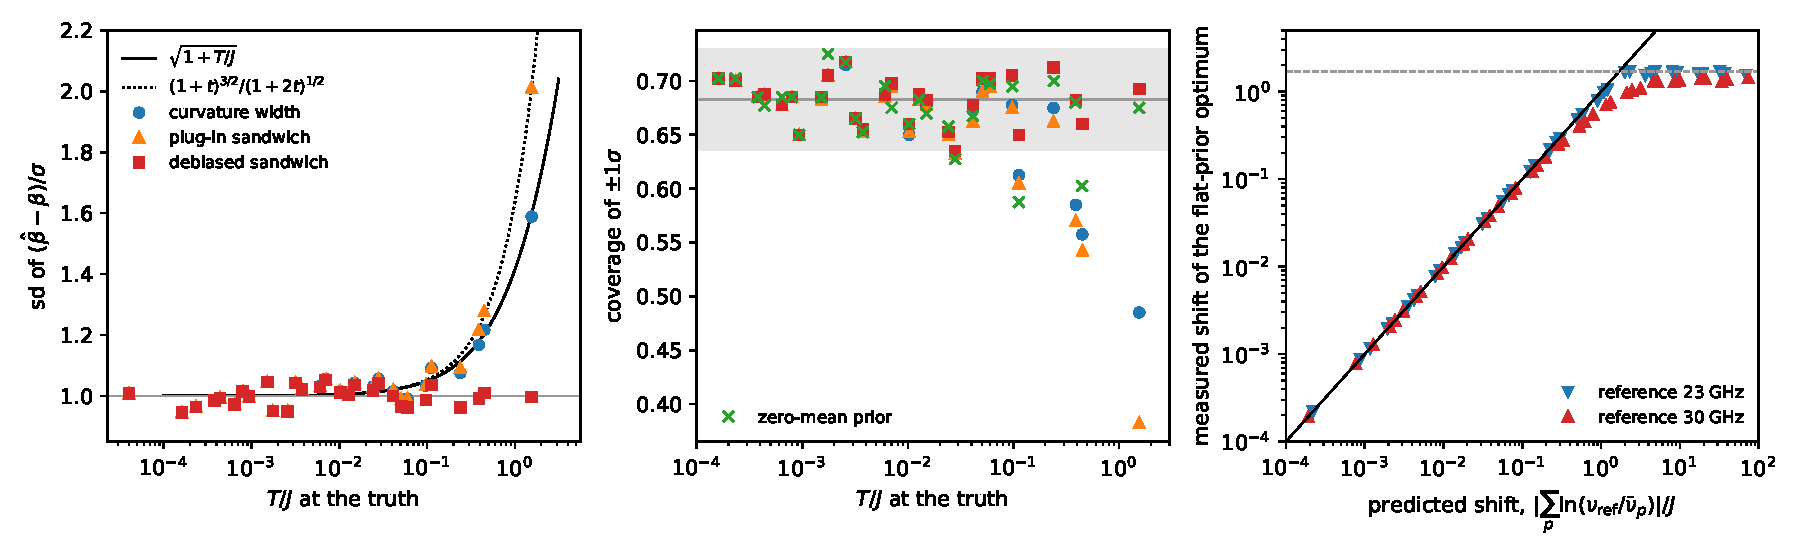
\includegraphics[width=\textwidth]{figures/fig_ladder.pdf}
\caption{One index shared by $n = 32$ to 8192 heavy-tailed amplitudes at five bands, per-amplitude
signal-to-noise ratio from 9 to 0.07, 400 noise realizations per cell; cells in which the index is
measured to better than 0.25 (\exref{E041}). Left: standard deviation of the standardized error of the
profile optimum with three error estimates, each taken from the same data set as the estimate, against
$\Tm/\J$ at the truth. The curvature width follows Eq.~(\ref{eq:sdz}) (line), the plug-in sandwich is
narrower still (dotted: its expected factor), and the debiased sandwich of Eq.~(\ref{eq:debiased})
stays at one. Centre: coverage of the $\pm1\sigma$ interval for the same three and for the zero-mean
prior; the band is $\pm2$ binomial standard errors around 0.683. Right: shift of the flat-prior
optimum from the profile optimum against the first-order prediction of Sect.~\ref{sec:flat}, at
references of 23 and 30 GHz, all 40 cells; the dashed line is the edge of the allowed range.}
\label{fig:ladder}
\end{figure}

Figure~\ref{fig:ladder} tests this over a ladder designed to reach the regime where it matters:
many faint amplitudes sharing one index, with predictions written down before the run
(\exref{E041}). With the curvature width the standard deviation of the standardized error equals
Eq.~(\ref{eq:sdz}) within 0.054 in all 30 cells where the index is measured, up to 1.59 at
$\Tm/\J = 1.56$, and 68 percent intervals cover the truth as rarely as 49 percent of the time. With
the plug-in sandwich they cover it 38 percent of the time. With Eq.~(\ref{eq:debiased}) the
standardized error has standard deviation 0.95 to 1.05 and the coverage is 0.65 to 0.72 in 29 cells
and 0.635 in one; the mean standardized error is within 0.10 everywhere. The coupled case with
several regions, three components and the dense WMAP covariances is tested in
Sect.~\ref{sec:data}.

\subsection{The zero-mean prior with a free scale}

The Bayesian relative of the profile likelihood is a zero-mean Gaussian amplitude prior with a
variance per index region that is inferred with the index. For a noise pattern that is common to the
amplitudes of a region, $w_{pb} = w_b$, the marginal likelihood depends on the data through
$q(\beta) = \sum_p b_p^2/A$ only, with $b_p = \sum_b w_b m_b d_{pb}$ and $A = \sum_b w_b m_b^2$, and
maximizing over $\tau$ gives
\begin{equation}
  \ln\mathcal{L}_{\tau}(\beta) = \tfrac12\, q(\beta) - \tfrac{n}{2}\ln q(\beta) + \mathrm{const}
  \qquad (q > n) ,
\end{equation}
a monotonic function of the profile log-likelihood $\tfrac12 q$. The optimum is the profile optimum,
and the curvature is the profile's times $1 - n/q$, which is the plug-in form of $1/(1+\Tm/\J)$. In
this case the zero-mean prior with a free scale \emph{is} the profile likelihood with its sandwich
width: the prior learns from the scatter of the fitted amplitudes how much of them is noise.
Simulation confirms the identity to the tolerance of the optimizer (\exref{E041}).

When the noise pattern varies between the amplitudes, as it does on real maps, the two estimators
part. The Gaussian prior is then a model for the amplitudes, real polarized amplitudes are far from
Gaussian, and the bright ones carry whatever noise pattern they happen to have. In the ladder the
resulting bias of the zero-mean prior is between $-0.6$ and $+0.3$ posterior standard deviations,
with a sign that belongs to the amplitude configuration and not to the noise level, while its
coverage stays within 0.59 to 0.73. On the realistic sky of Table~\ref{tab:flat} it was within 0.11
standard deviations except in one class at four times the real noise ($-0.30$; \exref{E036}). A scale
map in place of a single scale reduces it there. We therefore take the profile likelihood with the
debiased sandwich as the estimator of record and report the zero-mean prior beside it. What the
prior offers in exchange is a proper posterior, which a hierarchical model of an index field needs.

\subsection{What each target is good for}

\begin{table}
\centering
\caption{The index targets of Sect.~\ref{sec:model} for an index shared by many amplitudes, as
established by the experiments cited.}
\label{tab:targets}
\small
\begin{tabular}{p{3.2cm}p{3.6cm}p{3.6cm}p{4.2cm}}
\toprule
target & centre & width & depends on $\nuref$ \\
\midrule
flat-prior marginal (and Gibbs with flat amplitude priors) & shifted by
$\ln(\nuref/\nupiv)\,\sigma_1^2$ (\exref{E036}, \exref{E041}) & curvature & yes: tilt
$e^{n\beta\ln\nuref}$ \\
profile likelihood & unbiased (\exref{E036}, \exref{E041}) & curvature too narrow by
$\sqrt{1+\Tm/\J}$; debiased sandwich calibrated (\exref{E041}) & no \\
zero-mean prior, free scale per region & unbiased for a common noise pattern; up to 0.6 sd otherwise
(\exref{E041}) & calibrated where unbiased & no \\
re-solve move inside a Gibbs sweep & close to the profile optimum & too wide by $\sqrt{T}$,
Eq.~(\ref{eq:Tk}) (\exref{E035}) & no \\
\bottomrule
\end{tabular}
\end{table}

Table~\ref{tab:targets} collects the results. Two remarks on scope. First, for an index \emph{field}
with a hierarchical prior the profile likelihood is not enough at low signal to noise: the profile
maxima of faint regions scatter, and a hierarchy reads that scatter as field variance
(\exref{E012}). A proper amplitude prior is then needed, and its specification becomes part of the
model (Sect.~\ref{sec:limits}). Second, the statements above are for amplitudes that enter linearly
with known Gaussian noise. Beams, masks and a correlated-noise model that is itself uncertain change
the numbers, not the structure.

\section{Demonstration on the public polarization maps}
\label{sec:data}

This section does one thing: it applies the estimators of Sects.~\ref{sec:flat} and \ref{sec:profile}
to the same real maps, with the same regions, mask, bands and noise model, so that the difference
between their answers is the difference between the estimators and nothing else. It does not deliver
a polarized synchrotron index. Sect.~\ref{sec:moves} shows why not: at the statistical precision these
maps offer, analysis choices that are independent of the estimator move the index by as much as its
error or more.

\subsection{Data and model}

\paragraph{WMAP.} The nine-year low-resolution ($N_{\rm side}=16$) Stokes $Q$ and $U$ maps of the K,
Ka, Q and V bands \citep{bennett2013} with their released dense inverse noise covariance matrices,
which carry the time-correlated noise of the differential scan and de-weight the poorly constrained
transmission-imbalance modes \citep{jarosik2007,jarosik2011}. We checked them as released
(\exref{E038}): symmetric to $10^{-9}$, positive definite with no null space, a pixel noise of 2.0
to 2.2 $\muK$ in brightness temperature, and a few modes at multipoles 2 to 6 whose variance is 65 to
164 times the median. \citet{watts2023} argue from a joint reprocessing that these matrices do not
fully describe the large-scale uncertainty of the nine-year maps; we use them as released and test
the sensitivity to the modes they flag.

\paragraph{Planck.} The PR4 map at 353 GHz \citep{npipe} as the dust tracer. For it the per-pixel $Q/U$ covariance of the map file is combined over the
sub-pixels of each $N_{\rm side}=16$ pixel, and the map is the corresponding weighted average.

\paragraph{Spectra.} Each band enters through its measured bandpass. For WMAP every detector is given
unit response to a thermal spectrum and the detectors and radiometers of a band are averaged with
equal weights, which reproduces the per-radiometer effective frequencies of the WMAP team's routine
to 0.005 GHz, and the team's correction for the drift of the band centres over the mission (0.13
percent at K band) is applied. For a power law of index $-3.1$ the effective frequencies are 22.41,
32.66, 40.30 and 59.99 GHz for K to V and 28.09 GHz for the 30 GHz band. Delta bands at the nominal
WMAP frequencies would steepen a K to Ka index by about 0.06 (a calculation, not a fit). The 353 GHz
band cannot be a delta band: a modified blackbody with index 1.53 and temperature 19.6 K
\citep{planck2018xi} seen through the band is 1.12 to 1.14 times its value at 353.0 GHz, depending on
which bolometers are counted, so a delta band overstates the dust at every lower frequency by that
factor. We use the band of the polarization-sensitive bolometers.

\paragraph{Beams.} The low-resolution maps are pixel averages of maps with beams from $0.88^\circ$
(K) to $0.08^\circ$ (353 GHz). A noise-free simulation with index $-3.1$ everywhere, each band seen
through its own Gaussian beam, gives region indices biased flat by 0.005 to 0.011 for the WMAP bands
(\exref{E038}). We therefore bring every band to a common $1^\circ$ window with an invertible
operator on the $N_{\rm side}=16$ grid, $\mathsf{S}_b = 1 + \mathsf{Y}\,\mathrm{diag}(f_\ell - 1)\,
\mathsf{Y}^{+}$ with $f_\ell$ the ratio of the beam windows to multipole 47, transforming the data and
the covariance together. In the simulation the residual bias is below 0.0025, and on the real maps
the correction moves the four indices by 0.0068, 0.0025, 0.0085 and 0.0035 where the simulation
predicted 0.0070, 0.0030, 0.0088 and 0.0041 (measured with the white CMB prior, on an earlier set of
four regions and without a mask; \exref{E040}).

\begin{figure}
\centering
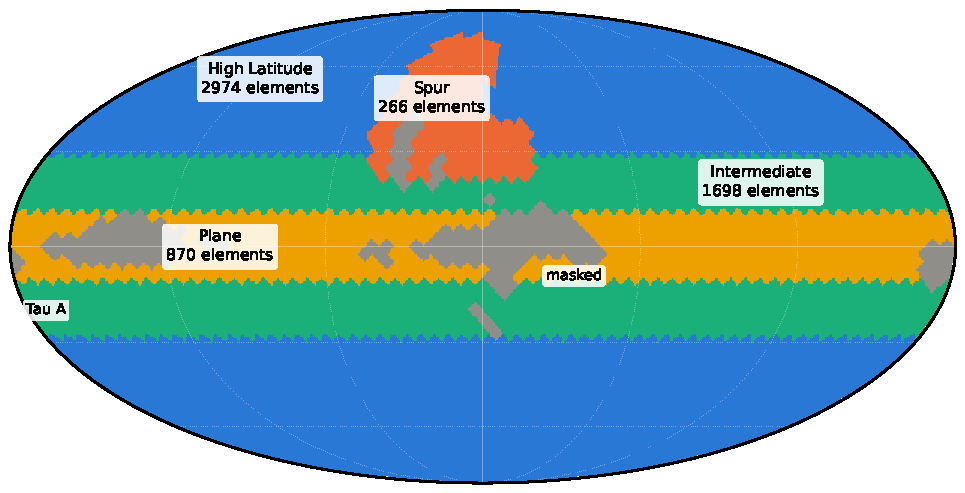
\includegraphics[width=0.85\textwidth]{figures/fig_regions.pdf}
\caption{The four regions and the processing mask (\exref{E044}), in Galactic coordinates with the Galactic
centre in the middle. An element is one Stokes parameter of one $N_{\rm side}=16$ pixel.}
\label{fig:regions}
\end{figure}

\paragraph{Regions and mask.} Four regions defined by geometry (Fig.~\ref{fig:regions}): \emph{High
Latitude}, $|b| > 30^\circ$; \emph{Intermediate}, $10^\circ \le |b| \le 30^\circ$; \emph{Plane},
$|b| < 10^\circ$; and \emph{Spur}, cut out of the first two, the northern part ($b > 20^\circ$,
$-45^\circ < l < 65^\circ$) of the pixels to which the released index map of \citet{svalheim2023}
gives its Spur value, which covers the North Polar Spur. A processing mask removes the 5 percent of
pixels with the largest polarized amplitude in the Cosmoglobe DR1 synchrotron model at 30 GHz smoothed
to $5^\circ$, which are the inner plane, the Fan region and the base of the Spur, and a disc of
$7.5^\circ$ around Tau A: \N{nkept} of \N{ntot} elements are kept, \N{nper.list} in the four regions.
\citet{svalheim2023} describe a mask of this kind for their index sampling (the strongest 5 percent of
the signal, and strong sources such as Tau A); ours follows that description and is not their file.
Masked elements are removed exactly: the kept elements enter with the inverse of their own block of
each covariance, the Schur complement of the full inverse covariance, formed after the window
matching. An earlier version of this analysis used four regions reconstructed from the released
index map without a mask; an independent referee showed that its ``High Latitude'' region held the
inner Galactic plane and that Tau A dominated the misfit of its ``Plane'' (Sect.~\ref{sec:moves}), and
those regions are not used for any statement below except where named.

\paragraph{Model.} Synchrotron as a power law with one index per region and one amplitude per
element (pixel and Stokes parameter); dust as the modified blackbody above with one amplitude per
element under a flat prior; and the CMB with one amplitude per element. The prior on the CMB
amplitudes is the $\Lambda$CDM covariance of $E$ and $B$ modes on the grid: spectra from CAMB
\citep{lewis2000} for the Planck 2018 parameters \citep{planck2018vi} with an optical depth of 0.054,
through the working window and the pixel window, for multipoles 2 to 47, the span of the harmonic
basis of the grid, plus a white floor of 0.01 $\muK$. The pixel average of a $\Lambda$CDM sky has a
further 0.11 $\muK$ per element from higher multipoles, nearly white, which this prior does not
describe (independent review, \exref{E040}); with the floor raised to that value the four indices
change by 0.0006 or less and their errors by 0.3 percent. Two other choices
are shown beside it, because the choice matters both for the index and for the pivot of
Sect.~\ref{sec:flat}: a white Gaussian prior of 0.2 $\muK$ per element, which we used first, and a
flat prior, for which the profile score is unbiased whatever the CMB is. The white prior has nearly
the right total variance (0.17 $\muK$ per element for $\Lambda$CDM) and the wrong shape: it
understates the $\Lambda$CDM $E$-mode variance by a factor of 200 at the quadrupole and overstates it
above multipole 10. With the mask, the prior on the kept elements is the kept block of that
covariance.

\paragraph{Expectations.} Expectations for every fit of this section were written down, with numbers,
before the fit was run, and the simulations of the next subsection were read before any real map
(\exref{E039}, \exref{E040}, \exref{E044}). The fits on the present regions were not the first look at
these maps: they follow a round on the earlier regions whose results we had seen, and the choice of
the $\Lambda$CDM prior over the white one was made by a rule written three minutes before the first
$\Lambda$CDM fit, after a referee had shown the white prior wrong in shape. The records mark what was
written when, and record the expectations that failed; several did, and the text says so where it
matters.

\subsection{Validation on simulations with the real covariances}

Before any fit to real data the chain was run on simulations with known indices: synchrotron
amplitudes from the Cosmoglobe DR1 polarized synchrotron map, dust amplitudes from the 353 GHz map,
a CMB drawn from the white prior, one true index per region chosen away from the centre of the allowed
range ($-3.15$, $-3.25$, $-2.85$, $-2.95$), and noise drawn from the real covariances
(\exref{E039}). Six criteria were fixed in advance. The simulations use the four regions of the earlier
version of this analysis as their geometry, and its names appear in Table~\ref{tab:e039} as labels
only; nothing tested here depends on what the regions are.

\begin{table}
\centering
\caption{Validation of the region-index estimators on simulations with the released WMAP noise
covariances (\exref{E039}): 200 noise realizations at $N_{\rm side}=8$, the first 40 with every
estimator. $z$ is the error of the profile optimum in units of the sandwich error at the truth.
The last block compares the difference between the flat-prior optima at 30 and 23 GHz with
Eq.~(\ref{eq:shift}) applied to each region alone and with the coupled form,
Eq.~(\ref{eq:coupled}), evaluated with $\J^{-1}$ in place of $\mathsf{H}^{-1}$ (the two agree here, where
$\Tm/\J$ is below 0.02).}
\label{tab:e039}
\small
\begin{tabular}{lrrrr}
\toprule
 & High Latitude & Spur & Galactic Center & Plane \\
\midrule
elements & 1124 & 212 & 50 & 150 \\
sandwich error at the truth & 0.0153 & 0.0166 & 0.0108 & 0.0146 \\
mean of $z$ & $-0.02 \pm 0.07$ & $0.00 \pm 0.07$ & $+0.07 \pm 0.07$ & $+0.01 \pm 0.07$ \\
standard deviation of $z$ & 1.04 & 0.98 & 0.94 & 1.02 \\
coverage of $\pm1\sigma$ & 0.670 & 0.715 & 0.685 & 0.695 \\
zero-mean prior minus profile, in $\sigma$ & $+0.03$ & $0.00$ & $+0.06$ & $+0.04$ \\
\midrule
flat prior at 23 GHz minus profile & $-0.0008$ & $0.0000$ & $-0.0002$ & $-0.0004$ \\
flat prior at 30 GHz minus profile & $+0.0680$ & $+0.0270$ & $+0.0074$ & $+0.0138$ \\
\quad in units of $\sigma$ & $+4.5$ & $+1.6$ & $+0.7$ & $+0.9$ \\
30 GHz minus 23 GHz, measured & $+0.0687$ & $+0.0270$ & $+0.0076$ & $+0.0142$ \\
\quad predicted, each region alone & $+0.0692$ & $+0.0156$ & $+0.0015$ & $+0.0085$ \\
\quad predicted, coupled, with $\J^{-1}$ & $+0.0723$ & $+0.0278$ & $+0.0078$ & $+0.0145$ \\
\bottomrule
\end{tabular}
\end{table}

Table~\ref{tab:e039} gives the outcome for the four regions at $N_{\rm side}=8$, where the simulated
sky is constant inside each pixel by construction. The profile optimum is unbiased to 0.07 standard
deviations, its sandwich error is right to 6 percent, the 68 percent intervals cover the truth 69
percent of the time, and the reduced $\chi^2$ at the optimum is $1.0006$ with a scatter of 0.022. A
spot check at the working resolution, $N_{\rm side}=16$, with 12 realizations gives a pooled
standardized error of mean $+0.03$ and standard deviation 0.99 and a reduced $\chi^2$ of $0.998 \pm
0.009$. The zero-mean prior lands within 0.06 standard deviations of the profile optimum. For this
band set with the white CMB prior the pivot sits at 23 GHz: a flat prior stated there is neutral, and
the same prior stated at 30 GHz moves the High Latitude index by 4.5 standard deviations. The
single-region formula predicts that move for the large region and fails for the three small ones,
which move by 1.7 to 5 times their own prediction: they are dragged by the large region through the
shared noise. The coupled form, Eq.~(\ref{eq:coupled}) with $\J^{-1}$, is within 5 percent in all four. Two of our
six criteria failed as written, one because it was worded wrongly (a lower bound of 1.0 on a ratio
that scatters around one) and one because it was written for the single-region formula. In these
regions $\Tm/\J$ is below 0.02, so the errors taken from each realization (Eq.~\ref{eq:debiased})
differ from the errors at the truth by less than a percent: with the errors taken from each of 40
realizations the standardized error has a standard deviation of 0.97 and the 68 percent coverage is
0.70, for the curvature, plug-in and debiased errors alike. The correction itself is tested in
Fig.~\ref{fig:ladder}, not here.
These simulations were first run on a numerical path that was later found to overwrite memory
(Sect.~\ref{sec:impl}); they were run again on a sound path and every number in
Table~\ref{tab:e039} and in this paragraph was reproduced to the last printed digit (\exref{E043}).

\subsection{The same maps, several answers}
\label{sec:same}

\begin{table}
\centering
\caption{The polarized synchrotron index of the WMAP nine-year K, Ka, Q and V maps (with Planck PR4
353 GHz for dust) in the four regions of \citet{svalheim2023}, at $N_{\rm side}=16$ with the dense
noise covariances, all bands brought to a common window, and the $\Lambda$CDM covariance as the prior
on the CMB (\exref{E040}). Top: the profile optimum with two errors, the debiased sandwich error,
which assumes one index per region (in parentheses for the Galactic Center, where that model does
not fit), and a block error from the scatter of the score over patches of sky, which does not (see
the text; none is quoted for the Galactic Center, where fewer than three patches carry the
information). Then the answer when the same likelihood is instead marginalized over flat
amplitude priors with the synchrotron amplitude defined at 23 or at 30 GHz, or under a zero-mean
prior with a free scale. Middle: the difference between the two flat-prior answers against
Eq.~(\ref{eq:coupled}). Bottom: goodness of fit, as $\chi^2$ per element and band, for which three
free amplitudes on five bands leave an expectation of 0.6.}
\label{tab:e040}
\small
% generated by nextgen/scripts/paperA1_make_tables.py; do not edit
\begin{tabular}{lrrrr}
\toprule
 & High Latitude & Spur & Galactic Center & Plane \\
\midrule
elements & 4388 & 928 & 182 & 646 \\
profile likelihood & $-3.082$ & $-3.080$ & $-3.081$ & $-2.964$ \\
\quad sandwich error & 0.012 & 0.016 & (0.009) & 0.013 \\
\quad block error & 0.044 & 0.038 &  & 0.100 \\
\quad effective number of patches & 5.7 & 8.8 & 2.5 & 5.1 \\
flat prior at 23 GHz & $-3.092$ & $-3.085$ & $-3.082$ & $-2.967$ \\
flat prior at 30 GHz & $-2.925$ & $-2.990$ & $-3.054$ & $-2.919$ \\
\quad minus profile, in units of the sandwich error & $+12.6$ & $+5.4$ & $+3.1$ & $+3.4$ \\
zero-mean prior, free scale & $-3.090$ & $-3.093$ & $-3.075$ & $-2.972$ \\
\midrule
flat 30 GHz minus flat 23 GHz & $+0.167$ & $+0.095$ & $+0.029$ & $+0.048$ \\
\quad Eq.~(\ref{eq:coupled}) & $+0.184$ & $+0.102$ & $+0.030$ & $+0.051$ \\
\midrule
$\chi^2$ per element and band & 0.58 & 0.59 & 1.78 & 0.77 \\
$\Tm/\J_{\rm c}$ & 0.014 & 0.005 & 0.0003 & 0.003 \\
\bottomrule
\end{tabular}

\end{table}

Table~\ref{tab:e040} is the result of this section. The numbers in each column come from the same
maps, the same regions, the same bands, the same bandpasses and the same noise covariances. They
differ only in how the amplitudes are removed.

Under flat amplitude priors the answer depends on where the amplitudes are defined. For this band set
with a $\Lambda$CDM prior on the CMB the pivot lies just above 23 GHz (23.3 to 23.4 GHz for the four
regions, to first order), and a flat prior stated at 23 GHz agrees with the profile optimum to 0.8
standard deviations. The same prior stated at 30 GHz gives
a High Latitude index of $-2.92$ instead of $-3.08$: flatter by 0.16, 12.6 standard deviations of
the sandwich error, with no change in the data or the model. The Spur moves by 0.09 and the Plane by
0.05. The difference between the two conventions is 0.91 to 0.95 of the first-order prediction,
Eq.~(\ref{eq:coupled}), in all four regions, so the identity of Sect.~\ref{sec:flat} holds on real
maps at the predicted size. The zero-mean prior with a free scale is within 0.8 standard deviations
of the profile optimum in every region.

\begin{table}
\centering
\caption{The fit of Table~\ref{tab:e040} under three priors on the CMB amplitudes: the
$\Lambda$CDM covariance, a white prior of 0.2 $\muK$ per element, and a flat prior (\exref{E040}).}
\label{tab:cmbprior}
\small
% generated by nextgen/scripts/paperA1_make_e044.py; do not edit
\begin{tabular}{lrrrr}
\toprule
 & High Latitude & Spur & Intermediate & Plane \\
\midrule
\multicolumn{5}{l}{\emph{profile likelihood, with the sandwich error}} \\
$\Lambda$CDM covariance & $-3.147 \pm 0.029$ & $-3.139 \pm 0.027$ & $-3.091 \pm 0.019$ & $-3.039 \pm 0.015$ \\
white, 0.2 $\mu$K & $-3.173 \pm 0.026$ & $-3.137 \pm 0.025$ & $-3.104 \pm 0.019$ & $-3.040 \pm 0.014$ \\
flat & $-3.041 \pm 0.062$ & $-3.122 \pm 0.060$ & $-3.017 \pm 0.044$ & $-3.038 \pm 0.035$ \\
\multicolumn{5}{l}{\emph{flat amplitude priors, synchrotron amplitude defined at 23 GHz}} \\
$\Lambda$CDM covariance & $-3.174$ & $-3.147$ & $-3.102$ & $-3.043$ \\
white, 0.2 $\mu$K & $-3.190$ & $-3.140$ & $-3.111$ & $-3.043$ \\
flat & $-1.600$$^\dagger$ & $-2.778$ & $-2.414$ & $-2.809$ \\
\multicolumn{5}{l}{\emph{flat amplitude priors, synchrotron amplitude defined at 30 GHz}} \\
$\Lambda$CDM covariance & $-2.696$ & $-2.993$ & $-2.898$ & $-2.971$ \\
white, 0.2 $\mu$K & $-2.775$ & $-3.046$ & $-2.934$ & $-2.975$ \\
flat & $-1.600$$^\dagger$ & $-2.577$ & $-1.737$ & $-2.519$ \\
\multicolumn{5}{l}{\emph{$\chi^2$ per element and band (expectation 0.60, 0.60 and 0.40)}} \\
$\Lambda$CDM covariance & 0.577 & 0.591 & 0.572 & 0.614 \\
white, 0.2 $\mu$K & 0.573 & 0.588 & 0.570 & 0.616 \\
flat & 0.385 & 0.408 & 0.372 & 0.385 \\
\bottomrule
\end{tabular}

\end{table}

\paragraph{The prior on the CMB.} The CMB has one amplitude per element like the other components,
and the index responds to what that amplitude is allowed to be (Table~\ref{tab:cmbprior}). We began
with a white prior of 0.2 $\muK$ per element and had fixed in advance that the $\Lambda$CDM covariance
would replace it if any index moved by more than one standard deviation between the two. The Plane
moved by 2.3 and the Spur by 1.0: with the white prior all four indices are steeper, by 0.012, 0.017,
0.006 and 0.031. A simulation says what to make of that (\exref{E040}): 60 skies with the synchrotron,
dust and noise of the validation above and a CMB drawn from the $\Lambda$CDM covariance, each fitted
with the three priors at $N_{\rm side}=8$. With the matched prior the estimate is unbiased and its
error is calibrated (standardized errors with mean $-0.15$ to $+0.11$ and standard deviation 0.93 to
1.14 by region). With the white prior it is unbiased on average, but the quoted error is too small by
24 to 32 percent in three of the four regions, and the 68 percent intervals cover 48 to 65 percent of
the time: the large-scale $E$ modes that a white prior does not allow move the estimate from sky to
sky, by 0.007, 0.009, 0.003 and 0.007 relative to the matched fit. With a flat prior the estimate is
unbiased and calibrated at 2.2 to 2.5 times the error. Measured against that sky-to-sky scatter and
its correlation between regions, the moves seen on the real maps at High Latitude, in the Spur and in
the Galactic Center are unremarkable (22 percent of the simulated skies lie further out), and the
move in the Plane is 4.4 standard deviations, which a $\Lambda$CDM sky does not do.
\pend{The same scatter at $N_{\rm side}=16$.} A white prior of the right total variance is therefore
not a harmless stand-in: it leaves the index unbiased and makes its error bar too small by a quarter
to a third before any misfit.

With a flat prior on the CMB the profile score is unbiased whatever the CMB is, at the price of errors
2.2 to 2.3 times larger, and the indices are $-3.03 \pm 0.03$, $-3.06 \pm 0.04$, $-3.01 \pm 0.02$ and
$-2.99 \pm 0.03$. Against the $\Lambda$CDM version, three regions are within the scatter that the
simulation gives for that difference (1.8, 0.7 and $-0.7$ of it) and the Galactic Center is 3.4 away.
The two regions whose index depends on the CMB prior by more than a $\Lambda$CDM sky allows are the
two that do not fit.

A free CMB amplitude also moves the pivot of Sect.~\ref{sec:flat}, and with it the size of the
convention effect. With a flat CMB prior and flat priors on the other amplitudes, the High Latitude
optimum of these same four WMAP bands is at $-2.51$ when the synchrotron amplitude is defined at 23
GHz and at $-1.71$ when it is defined at 30 GHz, where the profile likelihood says $-3.03 \pm 0.03$:
the pivot has moved below the K band (to 19.7 to 19.9 GHz, to first order), and both conventions
are far from it. The simulated band set of Table~\ref{tab:flat}, which includes the LFI bands, has its
pivots about 3 GHz higher in both cases and shows the same drop when the CMB is freed. The difference between
them, 0.80, is 0.92 of the first-order prediction, and the prediction is within 10 percent in every
region and for every prior in Table~\ref{tab:cmbprior}, for shifts between 0.03 and 0.8.

\paragraph{Errors that do not assume the model.} The sandwich error is the error of the estimator if
each region has one index and the noise model is right. The $\chi^2$ per element and band says that
this is close to true at High Latitude and in the Spur (0.58 and 0.59 against 0.6), 30 percent off in
the Plane and wrong by a factor of three in the Galactic Center. An error that does not lean on it
comes from the data: at the optimum the score of a region is a sum over elements, $\sum_p g_p = 0$,
and under the model the covariance of that sum is $\J + \Tm$; if the index varies inside the region
the partial sums over patches of sky scatter by more. With the 48 pixels of an $N_{\rm side}=2$ grid
as patches, $G_B = \sum_{p \in B} g_p$, the block covariance is
\begin{equation}
\widehat{\mathrm{Cov}}_{\rm block}(\hat\beta) = \J_{\rm c}^{-1}
\Big[\sum_B \frac{G_B G_B\T}{(1-h_B)^2}\Big] \J_{\rm c}^{-1},
\qquad h_B = \frac{D_B}{\sum_{B'} D_{B'}},
\label{eq:block}
\end{equation}
with $D_B = \partial G_B/\partial\beta$ the information carried by patch $B$. Without the factor
$(1-h_B)^{-2}$ this is the cluster sandwich in common use \citep{liang1986}, which is biased low when
a few clusters carry the information; with it, it is the leverage-corrected form that in linear
regression equals the delete-one-cluster jackknife variance up to a factor $G/(G-1)$ for $G$ clusters
\citep{bell2002,cameron2015}. Our estimator is not linear, so the correspondence holds to first
order, and it is exact only where neither the noise covariance nor the prior on the CMB couples
patches. Patches are treated as independent. The information is far from evenly spread: the number of
patches that would carry it if all carried the same, $(\sum_B D_B)^2/\sum_B D_B^2$ (an analogue, in
shares of the information, of the effective number of clusters of \citealt{carter2017}), is 6, 9, 3
and 5 for the four regions on the maps, out of 46, 29, 4 and 16 patches with data. A block error from
one sky is therefore itself uncertain by a third or so and should be read with the quantiles of a
$t$ distribution with few degrees of freedom \citep{bell2002,cameron2015}; for the Galactic Center we
quote none.

What a block error means needs care (independent review, \exref{E040}). It is the error of the
estimate as a measurement of the mean index of a population of exchangeable patches. For the
information-weighted mean index of the region as realized on this sky, the sandwich error is the
right one. If the index varies coherently over several patches the block error is too small (0.6 to
0.7 of the true scatter for a correlation length of two patches in a test by the reviewer). And if the
noise covariance or the prior couples patches, the patch scores are anticorrelated and the block
error is too large even when the model is true, so the ratio of block error to sandwich error under
the model has to be taken from simulations with the covariances and the prior of the fit. With
independent patches (white CMB prior, $N_{\rm side}=8$) the block error reproduces the scatter of the
estimate: the root mean square of the standardized error is 0.82, 1.20 and 1.02 at High Latitude, in
the Spur and in the Plane where 1.1 to 1.2 is expected, and the form without the leverage correction
is too small (1.39 and 1.26 in the Spur and the Plane). When the same simulations are given a true
spread of the index of 0.1 between patches, drawn anew for each realization, the sandwich error is too
small by a factor of 2.4 to 3.1 and the block error follows the scatter of the estimate about the mean
index of the region (0.59, 0.99 and 0.91). In that test the scatter of the estimate is, within 10
percent, the spread between patches divided by the square root of the effective number of patches,
added in quadrature to the sandwich error. The rule for choosing between this form and two others,
closest to one in both tests and in doubt the more conservative, was written before either test was
read; the three forms differ by 15 to 45 percent on the maps and all are in the record.

\begin{figure}
\centering
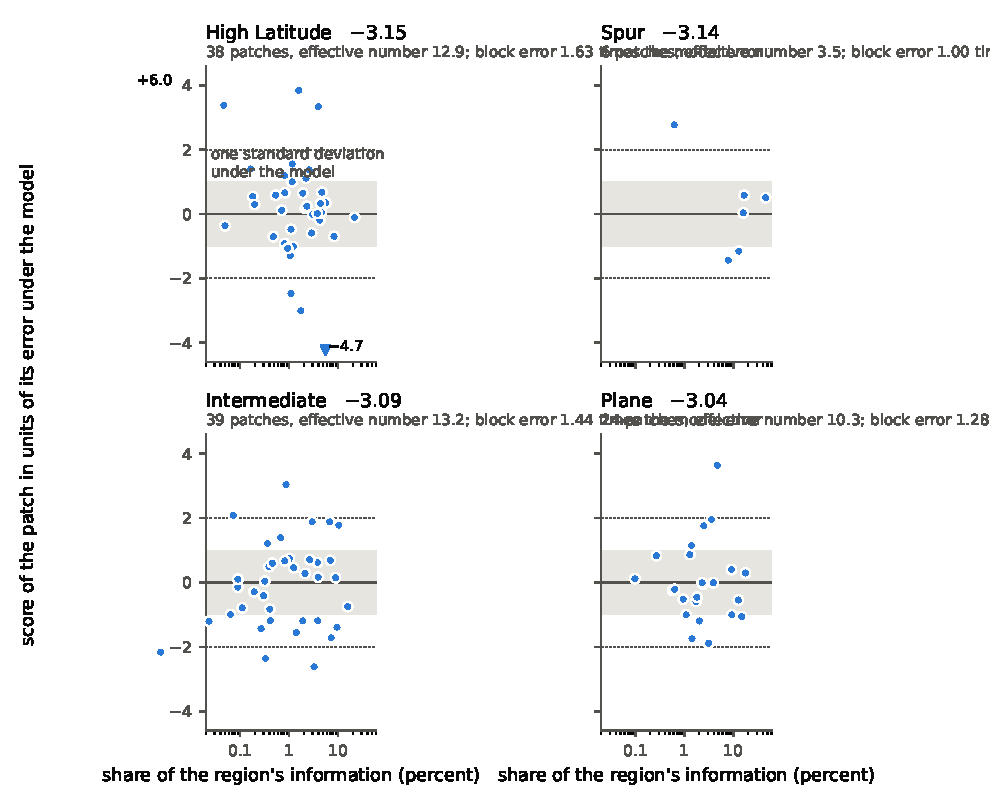
\includegraphics[width=\textwidth]{figures/fig_blocks.pdf}
\caption{What the block errors of Table~\ref{tab:e040} are made of. For each patch of sky (a pixel of the
$N_{\rm side}=2$ grid) that carries information on the index of a region: the index that the patch alone
would move to in one Newton step from the fitted index of the region, with the error it would have under
the model, against the share of the region's information that the patch carries. Patches with a one-step
error above 0.12 are not drawn, and arrows mark values outside the frame. Dark band: the sandwich error of
the region's index. Light band: its block error (none for the Galactic Center). The fitted index of the
region is given beside its name. The one-step values are first-order and for display; the block error
is computed from the scores, Eq.~(\ref{eq:block}) (\exref{E040}).}
\label{fig:blocks}
\end{figure}

On the maps the block error is 3.5, 2.3 and 7.5 times the sandwich error at High Latitude, in the
Spur and in the Plane (Table~\ref{tab:e040}, Fig.~\ref{fig:blocks}): 0.04, 0.04 and 0.10 where the
model gives 0.012, 0.016 and 0.013. Under the model, with the window-matched covariances and the $\Lambda$CDM prior of the fit, the ratio is
not one: in 60 simulations at $N_{\rm side}=8$ its median is 1.28, 1.21 and 1.32 and its largest value
2.8, 2.4 and 2.8, because that prior couples the patches (with the white prior the medians are 1.25,
1.03 and 1.07). Against that reference the maps are outside the range at High Latitude and in the
Plane, and the Spur is inside it: one simulation of 60 has a larger ratio. \pend{The same reference at
$N_{\rm side}=16$.} So the High Latitude region and the Plane are not one index each; for the Spur the
block error is an upper limit on the error and no evidence of misfit. In the simulation with a spread of 0.1 the median ratio is 3.8, 2.4 and 3.6. (That simulation has the
white prior; a spread of that size is the scale of what the High Latitude ratio asks for, and the
Plane asks for more.) What the fit of a region returns is the index of the half dozen patches that
carry its information. With the block errors the four regions do not differ from each other.

The comparison between the rows of Table~\ref{tab:e040} is differential. It does not need the model
to be right, only to be the same in every row.

\subsection{What moves the index, and why we do not quote one}
\label{sec:moves}

\begin{table}
\centering
\caption{Changes of the profile index of the WMAP K to V fit of Table~\ref{tab:e040} under analysis
choices that have nothing to do with the estimator (\exref{E040}, \exref{E042}). ``Index from $\ell \le
L$'': K band and 353 GHz keep all their modes, which with the prior on the CMB fixes the amplitudes,
and Ka, Q and V inform the
index through their harmonic coefficients at multipoles 2 to $L$ only. The window row compares two fits
with the white CMB prior, and the last row is the K, Ka fit minus the four-band fit when both are read
from multipoles up to 20. The flat-prior row repeats Table~\ref{tab:e040}. The statistical error of the
baseline is given for scale.}
\label{tab:moves}
\small
% generated by nextgen/scripts/paperA1_make_tables.py; do not edit
\begin{tabular}{lrrrr}
\toprule
 & High Latitude & Spur & Galactic Center & Plane \\
\midrule
baseline: all scales, $\Lambda$CDM CMB prior & $-3.082$ & $-3.080$ & $-3.081$ & $-2.964$ \\
statistical error (sandwich) & 0.012 & 0.016 & 0.009 & 0.013 \\
\midrule
flat amplitude prior at 30 GHz (Table~\ref{tab:e040}) & $+0.158$ & $+0.090$ & $+0.027$ & $+0.045$ \\
no window matching (white CMB prior, against its own baseline) & $+0.007$ & $+0.002$ & $+0.009$ & $+0.004$ \\
CMB prior: white, 0.2 $\mu$K & $-0.012$ & $-0.017$ & $-0.006$ & $-0.031$ \\
CMB prior: flat & $+0.055$ & $+0.025$ & $+0.073$ & $-0.024$ \\
index from $\ell \le 30$ & $-0.017$ & $-0.017$ & $-0.045$ & $-0.055$ \\
index from $\ell \le 20$ & $-0.024$ & $-0.031$ & $-0.055$ & $-0.084$ \\
index from $\ell \le 12$ & $-0.055$ & $-0.032$ & $-0.093$ & $-0.110$ \\
K and Ka only & $+0.024$ & $+0.012$ & $+0.038$ & $-0.002$ \\
dust index 1.48 in place of 1.53 & $-0.012$ & $-0.008$ & $-0.004$ & $-0.027$ \\
dust index 1.58 & $+0.011$ & $+0.007$ & $+0.004$ & $+0.025$ \\
no bandpass drift correction & $-0.001$ & $-0.001$ & $-0.001$ & $-0.001$ \\
353 GHz: all bolometers & $+0.002$ & $+0.001$ & $+0.001$ & $+0.003$ \\
delta bandpasses at the nominal frequencies & $-0.061$ & $-0.057$ & $-0.051$ & $-0.076$ \\
K and Ka only, both from $\ell \le 20$ (against the row above for $\ell \le 20$) & $+0.014$ & $+0.024$ & $+0.029$ & $+0.009$ \\
\bottomrule
\end{tabular}
% CMB prior: white, 0.2 $\mu$K: value -3.0940 -3.0965 -3.0867 -2.9950; sd 0.0121 0.0149 0.0088 0.0120; move in baseline sd -0.9 -1.0 -0.7 -2.3
% CMB prior: flat: value -3.0277 -3.0548 -3.0082 -2.9881; sd 0.0288 0.0358 0.0200 0.0300; move in baseline sd +4.4 +1.5 +8.2 -1.8
% index from $\ell \le 30$: value -3.0998 -3.0973 -3.1258 -3.0187; sd 0.0138 0.0177 0.0100 0.0147; move in baseline sd -1.4 -1.1 -5.1 -4.1
% index from $\ell \le 20$: value -3.1062 -3.1106 -3.1354 -3.0483; sd 0.0151 0.0190 0.0111 0.0156; move in baseline sd -1.9 -1.9 -6.2 -6.3
% index from $\ell \le 12$: value -3.1379 -3.1124 -3.1739 -3.0742; sd 0.0192 0.0207 0.0134 0.0168; move in baseline sd -4.4 -2.0 -10.5 -8.3
% K and Ka only: value -3.0583 -3.0683 -3.0431 -2.9664; sd 0.0159 0.0207 0.0115 0.0170; move in baseline sd +1.9 +0.7 +4.3 -0.2
% dust index 1.48 in place of 1.53: value -3.0949 -3.0879 -3.0850 -2.9916; sd 0.0126 0.0165 0.0089 0.0135; move in baseline sd -1.0 -0.5 -0.5 -2.1
% dust index 1.58: value -3.0713 -3.0726 -3.0769 -2.9395; sd 0.0124 0.0164 0.0088 0.0131; move in baseline sd +0.9 +0.4 +0.4 +1.9
% no bandpass drift correction: value -3.0837 -3.0810 -3.0819 -2.9655; sd 0.0125 0.0165 0.0089 0.0133; move in baseline sd -0.1 -0.1 -0.1 -0.1
% 353 GHz: all bolometers: value -3.0809 -3.0789 -3.0802 -2.9607; sd 0.0125 0.0165 0.0088 0.0133; move in baseline sd +0.1 +0.1 +0.1 +0.3
% delta bandpasses at the nominal frequencies: value -3.1438 -3.1371 -3.1319 -3.0398; sd 0.0129 0.0170 0.0091 0.0138; move in baseline sd -4.9 -3.5 -5.8 -5.7
% K, Ka against four bands at l <= 20, in units of sqrt(sd_sub^2 - sd_full^2): +1.3 +1.8 +3.4 +0.8
% start at -2.7: change -0.00000 -0.00000 -0.00000 +0.00000

\end{table}

% generated by nextgen/scripts/paperA1_make_tables.py (prose template there; numbers from the result files)
Table~\ref{tab:moves} lists what else moves the answer in the central configuration. The rows are
changes of the index; the statistical error of the baseline is given for scale.

\paragraph{Angular scale.} To ask at which scales two bands disagree we first marginalized the modes of
one map at multipoles 2 to $L$ and refitted, with the same cut in the K, Ka fit as a control fixed in
advance, where nothing should move. The control failed: the K, Ka index moved toward flat in every
region, by $+0.08$, $+0.16$, $+0.11$ and $+0.37$ at $L = 20$ (white CMB prior; \exref{E042}). Read from
the other side, with the pixel scale excluded and the index informed by multipoles up to 30, 20 or 12
only, the four-band index steepens (Table~\ref{tab:moves}): by 0.017 to 0.055 at High
Latitude, 0.017 to 0.032 in the Spur, 0.045 to 0.093 in the Galactic Center
and 0.055 to 0.110 in the Plane. The estimator is sound: on simulations with known indices it
is unbiased and calibrated (standardized errors of standard deviation 0.95 to 1.03 over 100
realizations at $N_{\rm side}=8$), an independent review re-derived it and confirmed it on its own
simulations, and the difference between the large-scale and the all-scale estimate of one simulated
sky has zero mean and a spread of 0.9 to 1.1 times $(\sigma_{\rm low}^2 - \sigma_{\rm all}^2)^{1/2}$
(\exref{E039}). On the maps the differences at $L = 20$ are 2.8, 3.3, 8.2 and 10.4 times that number. The
shifts are the same within 0.025 with the white CMB prior. So the dependence on scale is a property of
these maps under this model, in every region, and not of the estimator or of the CMB prior. An index
read from the three cuts is not stable either: the largest difference between two cuts is
2.8, 2.0, 5.4 and 6.7 times the standard deviation expected for nested fits.

We do not know the cause. One candidate is instrumental: the maps are pixel averages of skies that are
not band-limited, structure below the pixel scale folds into it through each band's own beam, K band
has the widest, and the window operator works to multipole 47 with Gaussian beams. Against it, the one
simulation we have of sub-pixel structure leaves a residual of 0.002, though that sky had no compact
sources. The other candidate is the sky: compact structure in the plane may be flatter than the diffuse
emission, and an index that varies from patch to patch (previous subsection) makes an index from
large scales and an index from all scales weight the sky differently. \citet{fuskeland2014}, with maps
smoothed to a common $1^\circ$ beam before any pixel averaging, find $-2.98 \pm 0.01$ in the plane,
close to our all-scale K, Ka value there ($-2.97$) and not to the large-scale one ($-3.04$ at
$L = 20$); that favours the sky. The rows of Table~\ref{tab:moves} are sizes of an effect and not
corrections.

\paragraph{Band subset.} K and Ka alone give indices that differ from the four bands together by
$+0.024$, $+0.012$, $+0.038$ and $-0.002$. The two fits share K and Ka, so the standard deviation of their difference
under the model is $(\sigma_{\rm sub}^2 - \sigma_{\rm full}^2)^{1/2}$, and the differences are
$+2.5$, $+0.9$, $+5.2$ and $-0.2$ of it; with both fits read from multipoles up to 20 they are
$+1.3$, $+1.8$, $+3.4$ and $+0.8$. With the white CMB prior the shifts were larger and all of one
sign ($+0.032$, $+0.023$, $+0.041$ and $+0.015$). What remains with the $\Lambda$CDM prior is a flatter K
to Ka index at High Latitude and in the Galactic Center, where the model does not fit in any case. A
spectrum that steepens with frequency would do this, and so would a dust model that predicts too much
polarized dust at 41 and 61 GHz from 353 GHz.

\paragraph{Dust.} The dust spectrum is fixed. Changing its index by 0.05 either way moves the
synchrotron index by 0.012, 0.008, 0.004 and 0.026, linearly ($\partial\beta_{\rm s}/\partial\beta_{\rm d} =
0.24$, $0.15$, $0.08$ and $0.52$): one statistical standard deviation at High Latitude
and two in the Plane, more than we had written down in advance for three of the four regions. With the
uncertainty of the Planck value, 0.02,
it is 0.005 at High Latitude and 0.010 in the Plane.

\paragraph{Bandpasses.} Leaving out the correction for the drift of the WMAP band centres changes the
index by 0.001, and taking the 353 GHz band of all bolometers in place of the
polarization-sensitive ones by 0.001 to 0.003. Replacing the measured bandpasses by delta functions at
the nominal WMAP frequencies steepens it by 0.051 to 0.076, 3.5 to 5.8 statistical standard
deviations: the effective frequency of K band for a spectrum this steep is 22.4 GHz, not 22.8.

\paragraph{Poorly measured modes.} The released K-band covariance has 20 eigenmodes with more than
ten times the median variance. Projecting all of them out moves the K, Ka index by 0.002 to 0.015
(white CMB prior). This tests the modes the matrix knows about, not the claim that it understates
them.

Taken together: for these maps and regions the profile index of the simple model is $-3.08$ at High
Latitude, in the Spur and in the Galactic Center and $-2.96$ in the Plane. Its error is 0.01 to 0.02
if each region has one index and 0.04 to 0.10 from the scatter between patches. It moves by
0.01 to 0.07 with the prior on the CMB, by 0.02 to 0.11 with the angular scales that
inform it, by up to 0.04 with the band subset, by 0.004 to 0.026 for 0.05 in the dust index, and by
0.05 to 0.08 if the bands are taken at their nominal frequencies. A number with an error bar that
means what it says needs a model in which a region is more than one index and the scale dependence
understood. That is a separate piece of work, and we do not quote an index here.



\section{Limits: when a proper amplitude prior is needed}
\label{sec:limits}

The profile likelihood settles the question for a handful of indices that the data determine. It
does not settle it for an index field with a hierarchical prior at low signal to noise, where a
proper amplitude prior is needed, and there the prior becomes a model component with failure modes
of its own. We list what we established, as limits on what the earlier sections recommend. All of it
is on simulations.

\paragraph{A scale shared across index regions on a scale map.} If the zero-mean prior takes its
scale from a map, $a_p \sim \mathcal{N}(0, (s\,g_p)^2)$ with one $s$ for the sky, a scale map that is
wrong differently in different regions biases their indices with a sign that again depends on the
reference frequency. On the sky of Table~\ref{tab:flat}, a map that is 30 percent high at
$|b| > 30^\circ$ moves the high-latitude indices by $-0.026$ at a 23 GHz reference, $+0.029$ at 30 GHz
and $0.000$ at the pivot (\exref{E036}). The effect is coherent over a zone and of the order of its
pooled error. One free scale per index region does not have it.

\paragraph{Template-tied priors in intensity.} For positive intensity amplitudes we implemented
$a_p \sim \mathcal{N}(\mu\, g_p, (s\, g_p)^2)$ with a template $g$ and inferred $\mu$ and $s$ per
component. This prior passes simulation-based calibration on data drawn from itself (600
replicates, \exref{E016}) and gives calibrated index fields down to index-pixel signal-to-noise
ratios below one. It is exact only for its own template-error law. A template error of the same
size with a different conditional law, such as a template that is the true amplitude divided by a
30 percent scatter, shifts the faint-sky dust index by 0.11 at four stated standard deviations
(\exref{E021}): regressing amplitudes on a noisy template is itself an errors-in-variables problem.
At high signal to noise with a template built from the data and a sky outside the model class
(PySM \texttt{d1s1}), the posterior runs away: the index removes the component from all bands but
one because that lowers the prior cost by more than it raises $\chi^2$ (\exref{E020}). At the
white-noise depth of the WMAP and LFI intensity maps with a 30 percent template error the field mean
is recovered ($-3.017$ against $-3.000$), but the inferred field does not beat a constant index in
pixel error on that sky, and the field hyperparameters fail a four-chain split-$\hat R$ criterion
(1.11 to 1.42) although every chain passes its own convergence check (\exref{E032}).

\paragraph{What follows.} An index field with inferred smoothness is a different paper. The
conclusion for this one is narrower: where the question is one index per region and the region is
measured, use the profile likelihood with the debiased sandwich; do not use a flat amplitude prior
unless the reference frequency is the pivot; and do not share one amplitude scale across index
regions on a template.

\section{Implementation and validation}
\label{sec:impl}

\paragraph{Commander4.} In our branch of Commander4 the spectral-index Metropolis step of the
per-pixel path takes a \texttt{likelihood} option. \texttt{marginal} evaluates
Eq.~(\ref{eq:Lflat}) and \texttt{ridge} Eq.~(\ref{eq:Lprof}) in the acceptance, with the
amplitudes integrated or maximized analytically per pixel in a compiled kernel; \texttt{conditional}
is the Gibbs step at fixed amplitudes; \texttt{resolve\_chisq} keeps the move of
Sect.~\ref{sec:legacy} with a warning; \texttt{auto} resolves to \texttt{ridge} where the kernel
applies and to \texttt{conditional} otherwise. Each exact option is tested against a grid evaluation
of its target in unit tests. End to end, a seven-rank run on simulated maps matched the exact profile
posterior within 0.03 posterior standard deviations with width ratios 0.94 and 0.97
(\exref{E006}); in that realization the target itself sat 1.9 and 3.7 standard deviations from the
input indices, which a 40-seed repetition showed to be scatter of the harness at its noise level and
not an offset (\exref{E037}). On real nside-64 intensity maps the \texttt{ridge} chain matched an independent grid
evaluation of its target with shifts of $-0.06 \pm 0.04$ and $+0.06 \pm 0.05$ standard deviations and
width ratios 0.96 and 0.94 for the two indices (\exref{E014}). On the same maps the conditional Gibbs
step has a standard deviation 180 times smaller than the marginal one for the synchrotron index and
did not move in 2000 iterations, while the collapsed chains mix in tens of iterations: collapsing the
amplitudes is needed for mixing as well as for the target. \pend{Simulation-based calibration of the
ridge and marginal modes in Commander4 itself (300 replicates) is not yet run.}

\paragraph{The low-resolution module.} The analysis of Sect.~\ref{sec:data} uses a separate, small
dense implementation (\texttt{nextgen/lowres}): band-averaged spectra from the instrument
bandpasses, the collapsed objectives of Sect.~\ref{sec:model} for several coupled regions with dense
noise covariances, analytic gradients, and $\J$ and $\Tm$ of Eq.~(\ref{eq:JT}). At
$N_{\rm side} = 16$ with three components the amplitude system has 18\,432 unknowns, and a profile fit
of four regions takes three to five minutes on a desktop machine. Unit tests
check the gradients against finite differences, the diagonal-noise closed forms, $\J$ and $\Tm$
against $\sum u V$ and $\sum V$, the sandwich against the scatter of 300 fits, the plug-in bias and
its correction, and the identity of Eq.~(\ref{eq:tilt}) to nine digits. The bandpass readers
reproduce the published LFI colour-correction ratios to $3\times10^{-4}$ and the HFI unit conversions
to 0.3 percent (\exref{E038}), and the per-radiometer effective frequencies of the WMAP team's own
routine to 0.005 GHz (\exref{E039}). An independent statistical review of the module, by a reviewer who derived the targets from the
stated model before reading our derivations, found no code defect; it corrected the response formula
of Sect.~\ref{sec:flat} (the curvature of the marginal in place of the profile information), the
condition under which the profile score is unbiased when a component carries a prior
(App.~\ref{app:sandwich}), and a docstring, and it measured the limits of the plug-in error quoted in
Sect.~\ref{sec:profile} (\exref{E039}, independent review).

\section{Discussion and conclusions}
\label{sec:concl}

\paragraph{What to do.} For a spectral index shared by many pixels with linear amplitudes and known
noise: (i) evaluate the profile likelihood or a proper marginal directly in the acceptance step, never
the $\chi^2$ at freshly drawn amplitudes; (ii) do not use a flat amplitude prior unless the amplitudes
are defined at the pivot frequency of the band set, which depends on the other components and their
priors, and say which reference frequency was used; (iii) quote the profile optimum with the
debiased sandwich error, Eq.~(\ref{eq:debiased}), and check $\Tm/\J_{\rm c}$; (iv) if a prior is put
on a component that does not depend on the index, state the sensitivity of the index to that prior's
variance; (v) model the difference between the beams of the bands, even at $3.7^\circ$ pixels, and
use measured bandpasses for every band including the dust tracer.

\paragraph{What it changes for published numbers.} \pend{Final numbers from Sect.~\ref{sec:data}: the
spread between conventions on the same maps against the spread of published values; the K band
against 30 GHz result.}

\paragraph{What we did not do.} All results are for maps, at low resolution, with one index per
region and Gaussian noise of known covariance. We did not treat time-ordered data, gain or bandpass
sampling, or an index field with inferred smoothness, for which a proper amplitude prior is needed
and has the failure modes of Sect.~\ref{sec:limits}. The real-map test of the tempering law rests on
an acceptance-noise factor measured from the log of the same chain; the forward prediction (widths of
13.1 and 13.6 profile widths with amplitudes stored as maps) has not been run. The LFI noise model is
empirical and isotropic. The misfit of the four-region model on real data is large
(Sect.~\ref{sec:data}), so the quoted statistical errors are lower limits for the regions as defined.

\paragraph{Reproducibility.} Every number in this paper comes from a script in the repository and an
experiment record that states the question, the predictions written before the run, the command and
the outcome, including the predictions that failed. The records are cited inline.

\appendix
\section{Score, curvature and sandwich for the profile likelihood}
\label{app:sandwich}

Let $\Pi = \M\A^{-1}\M\T\Ni$ be the projector onto the model space, so that
$\Pm = \Ni(1 - \Pi)$, $\Pm\M = 0$ and $\chimin = d\T\Pm d$. With $\M_r = \partial\M/\partial\beta_r$
and $\Pm_r = \partial\Pm/\partial\beta_r$, differentiating $\Pm\M = 0$ gives $\Pm_r\M = -\Pm\M_r$. The
score is $s_r = -\tfrac12 d\T\Pm_r d$. For $d = \M a + n$:
\begin{equation}
  s_r = -\tfrac12 a\T\M\T\Pm_r\M a - a\T\M\T\Pm_r n - \tfrac12 n\T\Pm_r n
      = (\M_r a)\T\Pm\, n - \tfrac12 n\T\Pm_r n ,
\end{equation}
because $\M\T\Pm_r\M = -\M\T\Pm\M_r = 0$. The first term has zero mean. The second has mean
$-\tfrac12\tr(\Pm_r\mathsf{N}) = \tfrac12\,\partial\,\tr(\Pi)/\partial\beta_r = 0$, since
$\tr\Pi = k$ for every $\beta$. So $\E[s_r] = 0$ for any true amplitudes: the profile score is
unbiased.

The variance of the first term is $(\M_r a)\T\Pm\mathsf{N}\Pm(\M_{r'}a) = (\M_r a)\T\Pm(\M_{r'}a) =
\J_{rr'}$, using $\Pm\mathsf{N}\Pm = \Pm$. The second term is a quadratic form in Gaussian noise,
uncorrelated with the first, with covariance $\tfrac12\tr(\Pm_r\mathsf{N}\Pm_{r'}\mathsf{N}) =
\tfrac12\tr(\Pi_r\Pi_{r'})$. Writing $\mathsf{G} = \A^{-1}\M\T\Ni$,
\begin{equation}
  \Pi_r = (1 - \Pi)\M_r\mathsf{G} + \M\A^{-1}\M_r\T\Ni(1 - \Pi) ,
\end{equation}
and since $\mathsf{G}(1-\Pi) = 0$ and $(1-\Pi)\M = 0$ the two squared terms vanish in the
trace and the cross terms give
\begin{equation}
  \tfrac12\tr(\Pi_r\Pi_{r'}) = \tr\!\big(\A^{-1}\M_r\T\Pm\,\M_{r'}\big) = \Tm_{rr'} .
\end{equation}
The expected curvature follows from differentiating the score once more:
$\E[\partial^2(\tfrac12\chimin)/\partial\beta_r\partial\beta_{r'}] = \J_{rr'}$. The estimator
$\hat\beta$ that solves $s(\hat\beta) = 0$ therefore has covariance $\J^{-1}(\J+\Tm)\J^{-1}$ to
leading order, Eq.~(\ref{eq:sandwich}).

A Gaussian prior on a component whose spectrum does not depend on the index (the CMB with variance
$\sigma_{\rm c}^2$ per element) fits in by minimizing over that component first: the result is the
flat-prior problem for the remaining components with noise covariance
$\mathsf{N} + \mathsf{C}\,\Lambda^{-1}\mathsf{C}\T$, with $\mathsf{C}$ the columns of the constrained component and
$\Lambda$ its prior precision. Everything above then holds in expectation over noise and over skies
of that component drawn from the prior, with its sample variance counted in $\J + \Tm$. It does not
hold for a prior variance that differs from the true one. If the true variance is $\kappa^2$ times
the prior variance, the expected gradient of $\tfrac12\chimin$ is $(\kappa^2 - 1)\,t$ (the expected
score is minus that) with $t_r = \tr(\Lambda\A^{-1}\M_r\T\mathsf{B}\T)$, $\mathsf{B} = \A^{-1}\M\T\Ni$,
$\A$ containing the prior precision, and the optimum is biased by $-(\kappa^2-1)\,\J^{-1}t$ to first
order. A single factor $\kappa^2$ describes a prior that is wrong in size; a prior that is wrong in
shape, as a white prior is for the CMB, needs the calculation mode by mode. Because $t_r$ is a sum over elements of one sign, the bias
in units of the standard deviation grows as the square root of the number of elements.

For a prior that is wrong in shape the same calculation gives Eq.~(\ref{eq:mismatch}). Write
$\mathsf{F} = [\M\ \mathsf{C}]$ for all columns, $\A = \mathsf{F}\T\Ni\mathsf{F}$ plus $\Lambda =
\mathsf{S}_{\rm w}^{-1}$ on the block of the constrained component, $\hat a = \mathsf{G} d$ with
$\mathsf{G} = \A^{-1}\mathsf{F}\T\Ni$, and $r = \mathsf{R} d$ with $\mathsf{R} = 1 - \mathsf{F}\mathsf{G}$
for the residual. The gradient of $\tfrac12\chimin$ is $g_r = -(\mathsf{F}_r\hat a)\T\Ni r$ with
$\mathsf{F}_r = \partial\mathsf{F}/\partial\beta_r$. With data $d = \M a + \epsilon$, $\epsilon = \mathsf{C} c + n$
and $\mathrm{Cov}(c) = \mathsf{S}_{\rm t}$,
\begin{equation}
  g_r = -(\mathsf{F}_r a)\T\Ni\mathsf{R}\,\epsilon - \epsilon\T\mathsf{G}\T\mathsf{F}_r\T\Ni\mathsf{R}\,\epsilon .
\end{equation}
Both terms have the expectations of the matched case when $\mathsf{S}_{\rm t} = \mathsf{S}_{\rm w}$ (zero mean,
variance $\J + \Tm$). The difference is linear in $\Delta = \mathsf{S}_{\rm t} - \mathsf{S}_{\rm w}$:
\begin{equation}
  \E[g_r] = -\tr\big[\Delta\,(\mathsf{F}_r\mathsf{Z})\T\,\Ni\mathsf{R}\mathsf{C}\big], \qquad
  \mathrm{Cov}(g_r, g_{r'}) \simeq \J_{rr'} + \Tm_{rr'} + \mathsf{q}_r\T\Delta\,\mathsf{q}_{r'}, \qquad
  \mathsf{q}_r = (\Ni\mathsf{R}\mathsf{C})\T\,\mathsf{F}_r a ,
\end{equation}
with $\mathsf{Z} = \mathsf{G}\mathsf{C} = \mathsf{E}_{\rm c} - \A^{-1}_{\cdot\,{\rm c}}\Lambda$ the response of the
fitted amplitudes to a unit amplitude of the constrained component ($\mathsf{E}_{\rm c}$ selects its
block). The mean is exact to the order of the sandwich; the covariance neglects the change of the
noise-noise term under the mismatch. The optimum is then biased by $-\J^{-1}\E[g]$ and has covariance
$\J^{-1}[\J + \Tm + \mathsf{q}\T\Delta\mathsf{q}]\J^{-1}$. Every matrix in these expressions is formed in the
fit; on real data $\J$ is replaced by $\J_{\rm c}$ and $a$ by $\hat a$.

For the fitted amplitudes $\hat a = a + e$ with $\mathrm{Cov}(e) = \A^{-1}$,
$\E[(\M_r\hat a)\T\Pm(\M_{r'}\hat a)] = \J_{rr'} + \tr(\A^{-1}\M_r\T\Pm\M_{r'}) = \J_{rr'} + \Tm_{rr'}$,
which gives Eq.~(\ref{eq:debiased}).

For one power-law component, delta bands and diagonal noise, $\M_r a$ has elements
$a_p m_b \ln(\nu_b/\nuref)$, the projector removes the component of $\ln\nu$ along the amplitude
direction, and $\J = \sum_p a_p^2 A_p V_p$, $\Tm = \sum_p V_p$ with $A_p = \sum_b w_{pb}m_b^2$ and
$V_p$ the weighted variance of $\ln\nu_b$ under the weights $w_{pb}m_b^2$, Eq.~(\ref{eq:uV}).

\begin{thebibliography}{99}
\bibitem[Alonso et al.(2017)]{alonso2017} Alonso, D., Dunkley, J., Naess, S., \& Thorne, B. 2017, Phys. Rev. D, 95, 043504 (arXiv:1608.00551)
\bibitem[Alquier et al.(2016)]{alquier2016} Alquier, P., Friel, N., Everitt, R., \& Boland, A. 2016, Stat. Comput., 26, 29 (arXiv:1403.5496)
\bibitem[Andersen et al.(2023)]{andersen2023} Andersen, K.~J., Herman, D., Aurlien, R., et al. 2023, A\&A, 675, A13 (BeyondPlanck XIII; arXiv:2201.08188)
\bibitem[Andrieu \& Roberts(2009)]{andrieu2009} Andrieu, C., \& Roberts, G.~O. 2009, Ann. Statist., 37, 697 (arXiv:0903.5480)
\bibitem[Ball et al.(2003)]{ball2003} Ball, R.~C., Fink, T.~M.~A., \& Bowler, N.~E. 2003, Phys. Rev. Lett., 91, 030201 (arXiv:cond-mat/0301179)
\bibitem[Bardenet et al.(2017)]{bardenet2017} Bardenet, R., Doucet, A., \& Holmes, C. 2017, J. Mach. Learn. Res., 18, 1 (arXiv:1505.02827)
\bibitem[Beaumont(2003)]{beaumont2003} Beaumont, M.~A. 2003, Genetics, 164, 1139
\bibitem[Bennett et al.(2013)]{bennett2013} Bennett, C.~L., Larson, D., Weiland, J.~L., et al. 2013, ApJS, 208, 20 (arXiv:1212.5225)
\bibitem[Ceperley \& Dewing(1999)]{ceperley1999} Ceperley, D.~M., \& Dewing, M. 1999, J. Chem. Phys., 110, 9812
\bibitem[Dickinson et al.(2009)]{dickinson2009} Dickinson, C., Eriksen, H.~K., Banday, A.~J., et al. 2009, ApJ, 705, 1607 (arXiv:0903.4311)
\bibitem[Dunkley et al.(2009)]{dunkley2009} Dunkley, J., Spergel, D.~N., Komatsu, E., et al. 2009, ApJ, 701, 1804 (arXiv:0811.4280)
\bibitem[Engel(1985)]{engel1985} Engel, B. 1985, Kwantitatieve Methoden, 19, 5
\bibitem[Eriksen et al.(2008)]{eriksen2008} Eriksen, H.~K., Jewell, J.~B., Dickinson, C., et al. 2008, ApJ, 676, 10 (arXiv:0709.1058)
\bibitem[Fuskeland et al.(2014)]{fuskeland2014} Fuskeland, U., Wehus, I.~K., Eriksen, H.~K., \& N{\ae}ss, S.~K. 2014, ApJ, 790, 104 (arXiv:1404.5323)
\bibitem[Huber(1967)]{huber1967} Huber, P.~J. 1967, in Proc. Fifth Berkeley Symp. Math. Statist. Probab., Vol. 1, 221--233
\bibitem[Jarosik et al.(2007)]{jarosik2007} Jarosik, N., Barnes, C., Greason, M.~R., et al. 2007, ApJS, 170, 263 (arXiv:astro-ph/0603452)
\bibitem[Jarosik et al.(2011)]{jarosik2011} Jarosik, N., Bennett, C.~L., Dunkley, J., et al. 2011, ApJS, 192, 14 (arXiv:1001.4744)
\bibitem[Jew \& Grumitt(2020)]{jew2019} Jew, L., \& Grumitt, R.~D.~P. 2020, MNRAS, 495, 578 (arXiv:1907.11426)
\bibitem[Medina-Aguayo et al.(2016)]{medina2016} Medina-Aguayo, F.~J., Lee, A., \& Roberts, G.~O. 2016, Stat. Comput., 26, 1187 (arXiv:1503.07066)
\bibitem[Neyman \& Scott(1948)]{neyman1948} Neyman, J., \& Scott, E.~L. 1948, Econometrica, 16, 1
\bibitem[Nicholls et al.(2012)]{nicholls2012} Nicholls, G.~K., Fox, C., \& Watt, A.~M. 2012, arXiv:1205.6857
\bibitem[O'Neill et al.(2000)]{oneill2000} O'Neill, P.~D., Balding, D.~J., Becker, N.~G., Eerola, M., \& Mollison, D. 2000, Appl. Statist., 49, 517
\bibitem[Planck Collaboration Int. LVII(2020)]{npipe} Planck Collaboration Int. LVII. 2020, A\&A, 643, A42 (arXiv:2007.04997)
\bibitem[Planck Collaboration X(2016)]{planck2015x} Planck Collaboration X. 2016, A\&A, 594, A10 (arXiv:1502.01588)
\bibitem[Planck Collaboration XI(2020)]{planck2018xi} Planck Collaboration XI. 2020, A\&A, 641, A11 (arXiv:1801.04945)
\bibitem[Stompor et al.(2009)]{stompor2009} Stompor, R., Leach, S., Stivoli, F., \& Baccigalupi, C. 2009, MNRAS, 392, 216 (arXiv:0804.2645)
\bibitem[Svalheim et al.(2023)]{svalheim2023} Svalheim, T.~L., Andersen, K.~J., Aurlien, R., et al. 2023, A\&A, 675, A14 (BeyondPlanck XIV; arXiv:2011.08503v2)
\bibitem[Watts et al.(2023)]{watts2023} Watts, D.~J., Basyrov, A., Eskilt, J.~R., et al. 2023, A\&A, 679, A143 (arXiv:2303.08095)
\bibitem[Weiland et al.(2022)]{weiland2022} Weiland, J.~L., Addison, G.~E., Bennett, C.~L., Halpern, M., \& Hinshaw, G. 2022, ApJ, 936, 24 (arXiv:2203.11445)
\bibitem[White(1982)]{white1982} White, H. 1982, Econometrica, 50, 1--25
\end{thebibliography}

\end{document}
